
%%% PREAMBLE 
\documentclass[9pt,lineno]{RandlettLab_elife}
%\nolinenumbers
% Use the onehalfspacing option for 1.5 line spacing
% Use the doublespacing option for 2.0 line spacing
% Please note that these options may affect formatting.
% Additionally, the use of the \newcommand function should be limited.

\usepackage{lipsum} % Required to insert dummy text
\usepackage[version=4]{mhchem}
\usepackage{siunitx}
\DeclareSIUnit\Molar{M}

%%%%%%%%%%%%%%%%%%%%%%%%%%%%%%%%%%%%%%%%%%%%%%%%%%%%%%%%%%%%
%%% ARTICLE SETUP
%%%%%%%%%%%%%%%%%%%%%%%%%%%%%%%%%%%%%%%%%%%%%%%%%%%%%%%%%%%%
\title{Molecular and functional mechanisms of long-term visual habituation in larval zebrafish}

\author[1]{Laurie-Anne Lamiré}
\author[2]{Martin Haesemeyer}
\author[3,4\authfn{1}]{Florian Engert}
\author[5\authfn{1}]{Michael Granato}
\author[1\authfn{1},*]{Owen Randlett}


\affil[1]{
Laboratoire MeLiS, UCBL - CNRS UMR52684 - Inserm U1314, Institut NeuroMyoGène, Faculté de Médecine et de Pharmacie, 8 avenue Rockefeller, 69008, Lyon, France 
}

\affil[2]{
The Ohio State University, Department of Neuroscience, Columbus, OH 43210, USA
}

\affil[3]{
Department of Molecular and Cellular Biology, Faculty of Arts and Sciences, Harvard University, Cambridge, MA 02138, USA
}

\affil[4]{
Center for Brain Science, Faculty of Arts and Sciences, Harvard University, Cambridge, MA 02138, USA
}
\affil[5]{
Department of Cell and Developmental Biology, University of Pennsylvania, Perelman School of Medicine, 421 Curie Blvd, Philadelphia, PA 19104, USA
}

\corr{owen.randlett@univ-lyon1.fr}{OR}


\contrib[\authfn{1}]{Equal contribution}

%\presentadd[\authfn{3}]{Department, Institute, Country}
%\presentadd[\authfn{4}]{Department, Institute, Country}
% \presentadd[\authfn{5}]{eLife Sciences editorial Office, eLife Sciences, Cambridge, United Kingdom}

%%%%%%%%%%%%%%%%%%%%%%%%%%%%%%%%%%%%%%%%%%%%%%%%%%%%%%%%%%%%
%%% ARTICLE START
%%%%%%%%%%%%%%%%%%%%%%%%%%%%%%%%%%%%%%%%%%%%%%%%%%%%%%%%%%%%

\begin{document}

\maketitle

\begin{abstract}
Long-term habituation allows animals to learn to ignore persistent but unimportant stimuli. Despite being the most basic form of learning, a consensus model on the underlying mechanisms has yet to emerge. We have exploited a visual habituation paradigm in larval zebrafish, where larvae will learn to reduce their reactions to abrupt global dimming (a dark flash). Using a drug-screening approach, we first identified pathways that potently altered habituation learning, including GABAergic inhibition, Melatonin and Estrogen signaling. To determine how habituation manifests at the circuit-level, we used whole-brain pERK and 2-photon Ca\textsuperscript{2+} imaging. These analyses identified 12 classes of neurons that differ in their stimulus response profile, rate of adaptation during learning, anatomical location, and GABAergic identity. By analyzing how GABA and Melatonin alter population activity, we propose a model for dark flash habituation in which the suppression of activity begins early in the visual pathway but downstream of the Retina. This suppression is mediated by GABAergic inhibitory motifs resulting in heterogeneous inhibition of distinct neuronal types in the dark flash circuit. Our results have identified multiple molecular pathways acting in functional cell types underlying a form of long-term plasticity in a vertebrate brain, and allow us to propose the first iteration of a model for how and where this learning process is encoded in individual neurons to shape learned behaviour. 
\end{abstract}


\section{Introduction}

\begin{figure}
\begin{fullwidth}
\begin{center}

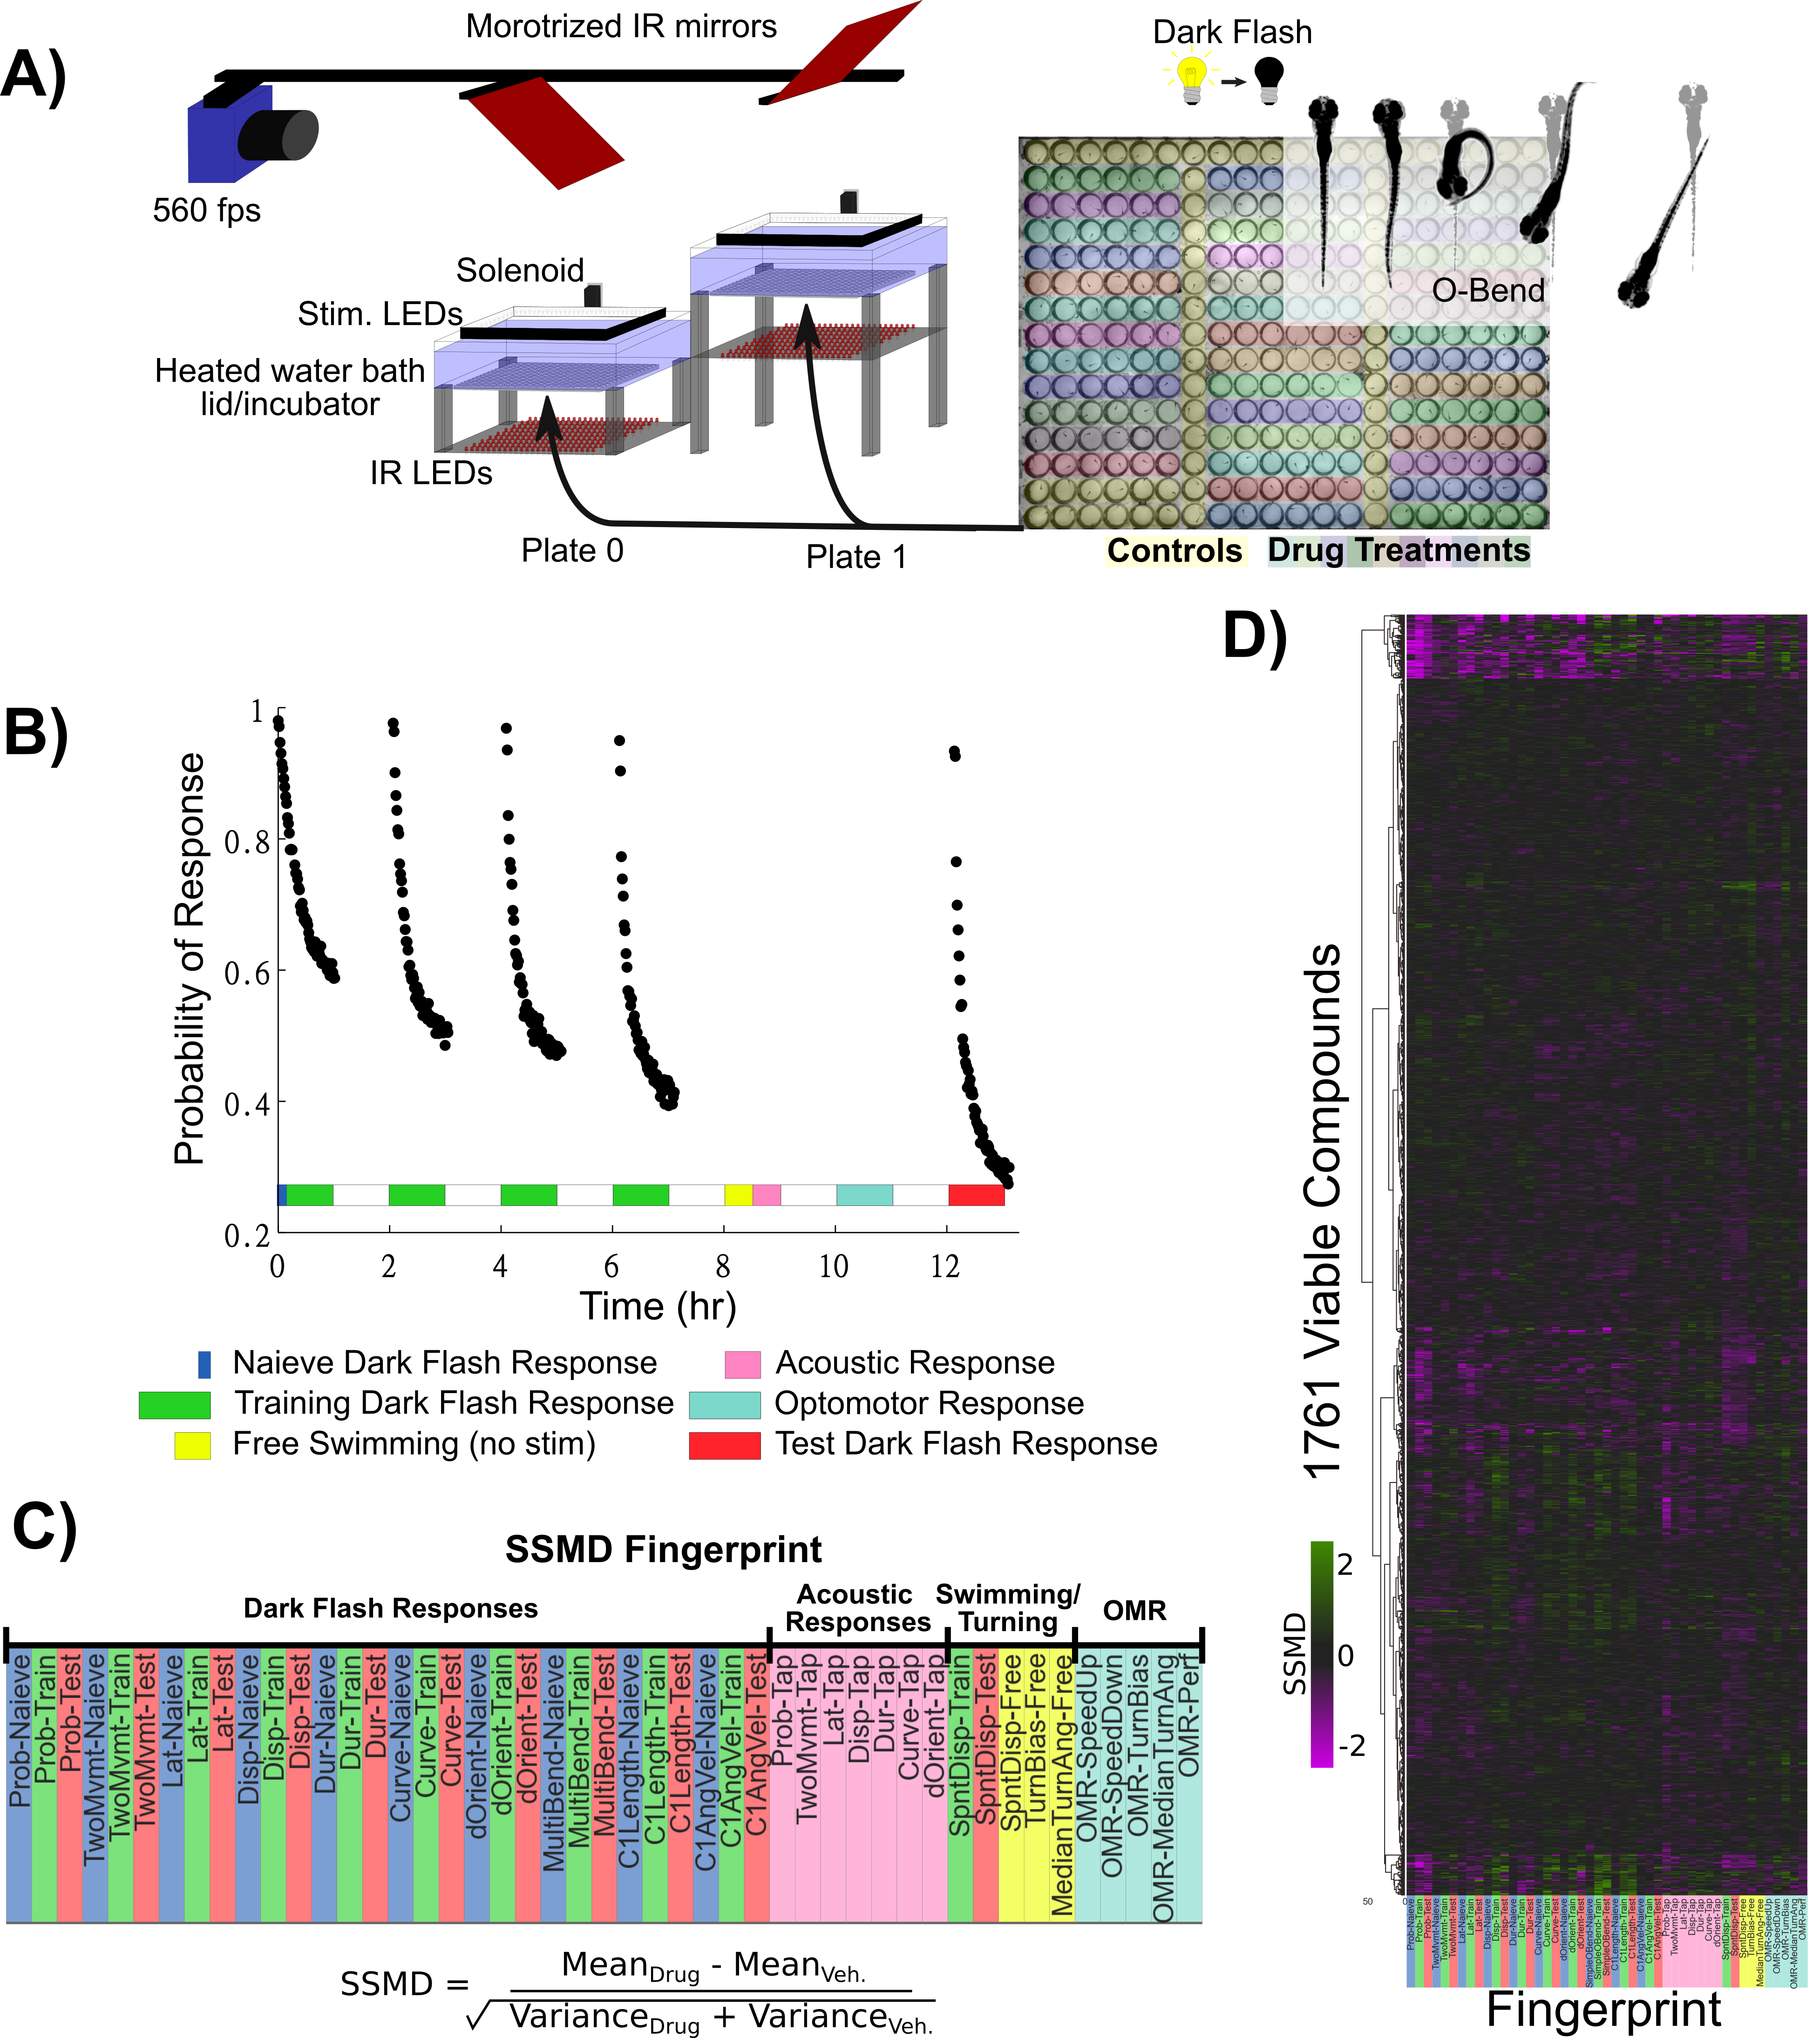
\includegraphics[width=0.8\linewidth]{Figure_1-ScreenSetup}
\caption{Pharmacological screening for dark flash habituation modulators. 
\textbf{A)} Screening setup to record larval zebrafish behaviour in 300-well plates, which are placed below a 31°C water bath that acts as a heated lid for the behaviour plates. Two 300-well plates are imaged in alternation using mirrors mounted on stepper motors. Fish are illuminated with infra-red LEDs and imaged with a high-speed camera recording at 560 frames per second (fps). Visual stimuli are delivered by a rectangular ring of RGB LEDs, and acoustic stimuli are delivered via a solenoid mounted on the back of the water tank. Colors overlaid on the 300-well plate indicate the arrangement of small molecule treatments and controls (yellow). 
\textbf{B)} Habituation results in a progressive decrease in responsiveness to dark flashes repeated at 1-minute intervals, delivered in 4 training blocks of 60 stimuli, separated by 1hr of rest (from 0:00-8:00. This epoch is separated into periods reflective of the naive response (first 5 stimuli, blue), and the remaining 235 stimuli during training (green). From 8:00-8:30, no stimuli are delivered and fish are monitored for spontaneous behaviour (yellow). From 8:30-9:00 fish are given acoustic stimuli via the solenoid tapping on the water bath (pink). From 10:00 - 11:00 fish are stimulated with alternating leftward and rightward motion using the RGB LEDs to induce the optomotor response and turning towards the direction of motion (light blue). Finally, at 12:00-13:00, larvae are given 60 additional dark flashes during the test period (red). 
\textbf{C)} The strictly standardized mean difference (SSMD) is calculated across these different time periods, behaviours and the different components of O-Bend behavioural habituation (Randlett et al., 2019). All drugs were dosed at 10 uM in 0.1\% DMSO (n = 6 larvae), relative to 0.1\% DMSO vehicle controls (n = 60 larvae). 
\textbf{D)} These vectors are assembled across all screened drugs that were viable and did not cause death or paralysis of the larvae. Displayed as a hierarchically clustered heatmap of behavioural Fingerprints (vectors of SSMD values). Clustering distance = ward, standardized euclidean. }
\label{fig:1}
\figdata{\href{https://github.com/owenrandlett/lamire_2022/blob/main/TableS1_Drugs_all_info.csv}{Small molecule library}, Selleckchem Bioactive: 2100 FDA-approved/FDA-like small molecules}
\label{table:1}
\figdata{\href{https://github.com/owenrandlett/lamire_2022/blob/main/TableS2_Drugs_Fingerprints.csv}{Behavioural fingerprints} for viable compounds}
\label{table:2}

\end{center}
\end{fullwidth}
\end{figure}

A central function of the brain is to change with experience: learning from the past to adapt behaviours in the now. At a base level, these adaptations can reflect attempts to identify and attend preferentially to salient stimuli. For example, identifying the smell of a predator or prey may be crucial, while identifying that my home still smells like my kin is not. This ability to suppress responses to continuous stimuli is known as habituation, and is generally considered to be the simplest form of learning and memory \cite{Rankin2009-er}. Habituation is conserved across all animals, and like other forms of plasticity, exists in at least two mechanistically distinct forms: transient short-term habituation, and protein-synthesis dependent long-term habituation. Here we focus on long-term habituation, which serves as a pragmatic model to dissect the molecular and circuit mechanisms of stably encoded plasticity processes in neural circuits. 

In recent years, a renewed focus on long-term habituation has led to significant insights into the adaptations underlying this process \cite{Cooke2020-mz, McDiarmid2019-mh}, nonetheless a consensus model on the general principles underlying habituation is yet to emerge.  Physiological and genetic work in Aplysia, and C. elegans were consistent with a model in which homosynaptic depression of excitatory synapses drives habituation \cite{Bailey1983-ei, Rose2003-dl} (although see \cite{Glanzman2009-tz}). In contrast, recent work in the \emph{Drosophila} olfactory and gustatory systems indicate that the potentiation of inhibitory neurons drives habituation rather than depression of excitatory connections \cite{Das2011-gd, Paranjpe2012-ce, Trisal2022-pa},  and habituation to specific orientations of visual cues in mice is associated with the potentiation of neuronal activity and synapses in the visual cortex \cite{Cooke2015-qs}, which requires GABAergic interneurons \cite{Kaplan2016-qk}. These studies are more consistent with a model in which the potentiation of inhibition, rather than depression of excitation, drives habituation \cite{Cooke2020-mz}. 

Recently, we found that long-term habituation of the response of larval zebrafish to sudden pulses of whole-field darkness, or dark flashes (DFs), involves multiple molecularly independent plasticity processes that act to suppress different components of the behavioural response \cite{Randlett2019-fi}. Similar behavioural, pharmacological, and genetic experiments have led to comparable conclusions in acoustic short-term habituation \cite{Nelson2022-qr}, and habituation in C. elegans \cite{McDiarmid2019-lo, McDiarmid2019-mh}, indicating that habituation generally acts via multiple modular plasticity processes. These modules act to mute or shift behavioural responses to repeated stimuli. How and where these processes are implemented in the circuit, and how conserved or derived these processes are across species or habituation paradigms remains to be determined. 

Here we have used a combination of high-throughput behavioural analyses, pharmacology and whole brain imaging to propose a model of DF habituation. By combining knowledge about critical neurotransmitters derived from pharmacology, with knowledge about functional classes of neurons derived from whole-brain imaging, we have established a model constrained on multiple scales.


\section{Results}
\subsection{Pharmacological screening strategy}

When stimulated with a dark flash (DF), larval zebrafish execute an O-bend response. The O-bend is characterised by a strong body bend and a large angle turning maneuver that forms part of the photactic strategy of larval zebrafish, helping them navigate towards lit environments \cite{Burgess2007-gq, Chen2014-qq}. When trained with repeated DFs, larvae will habituate and reduce their responsiveness in multiple independent ways, including: decreasing response probability, increasing latency, and decreasing multiple measures of response magnitude \cite{Randlett2019-fi}. As the molecular mechanisms leading to this form of habituation learning are still largely unknown, we used a pharmacological screening approach with the goal of identifying important molecular players in habituation. We used the high-throughput assay we previously established, which has a maximum throughput of 600 larvae/day (\autoref{fig:1}A, \cite{Randlett2019-fi}). As we aimed to identify modulators specific for habituation, we included additional behavioural assays as controls, including the response to acoustic stimuli, the optomotor response, and the spontaneous swimming behaviour of the fish in the absence of stimulation (\autoref{fig:1}B,C). 

Behavioural records for fish treated with each compound were compressed into a fingerprint \cite{Rihel2010-pj} -- a vector representing the strictly standardised mean difference (SSMD) across 47 aspects of behaviour (see Methods). For measurements related to dark-flash habituation behaviour, responses were time-averaged across three epochs chosen to highlight changes in habituation: the naive response (first 5 dark flashes), the response during the remaining training flashes, and the re-test block 5 hrs after training (\autoref{fig:1}B). This was done across 10 different components of the dark flash response (Probability of Response, Latency, Displacement, etc.). 


In each 300-well plate, 40 groups of 6 larvae were treated in individual wells, and compared to 60 vehicle treated controls (\autoref{fig:1}A). We chose these numbers based on a sub-sampling analysis that determined these numbers were sufficient to identify the effect of a known modulator of habituation (haloperidol \cite{Randlett2019-fi}) at a false-negative rate of less than 0.05 (not shown), while allowing us to screen 80 drugs per experiment across 2 plates (\autoref{fig:1}A). 


\subsection{Correlational structure in the pharmaco-behavioural space }

\begin{figure}
\begin{fullwidth}
\begin{center}
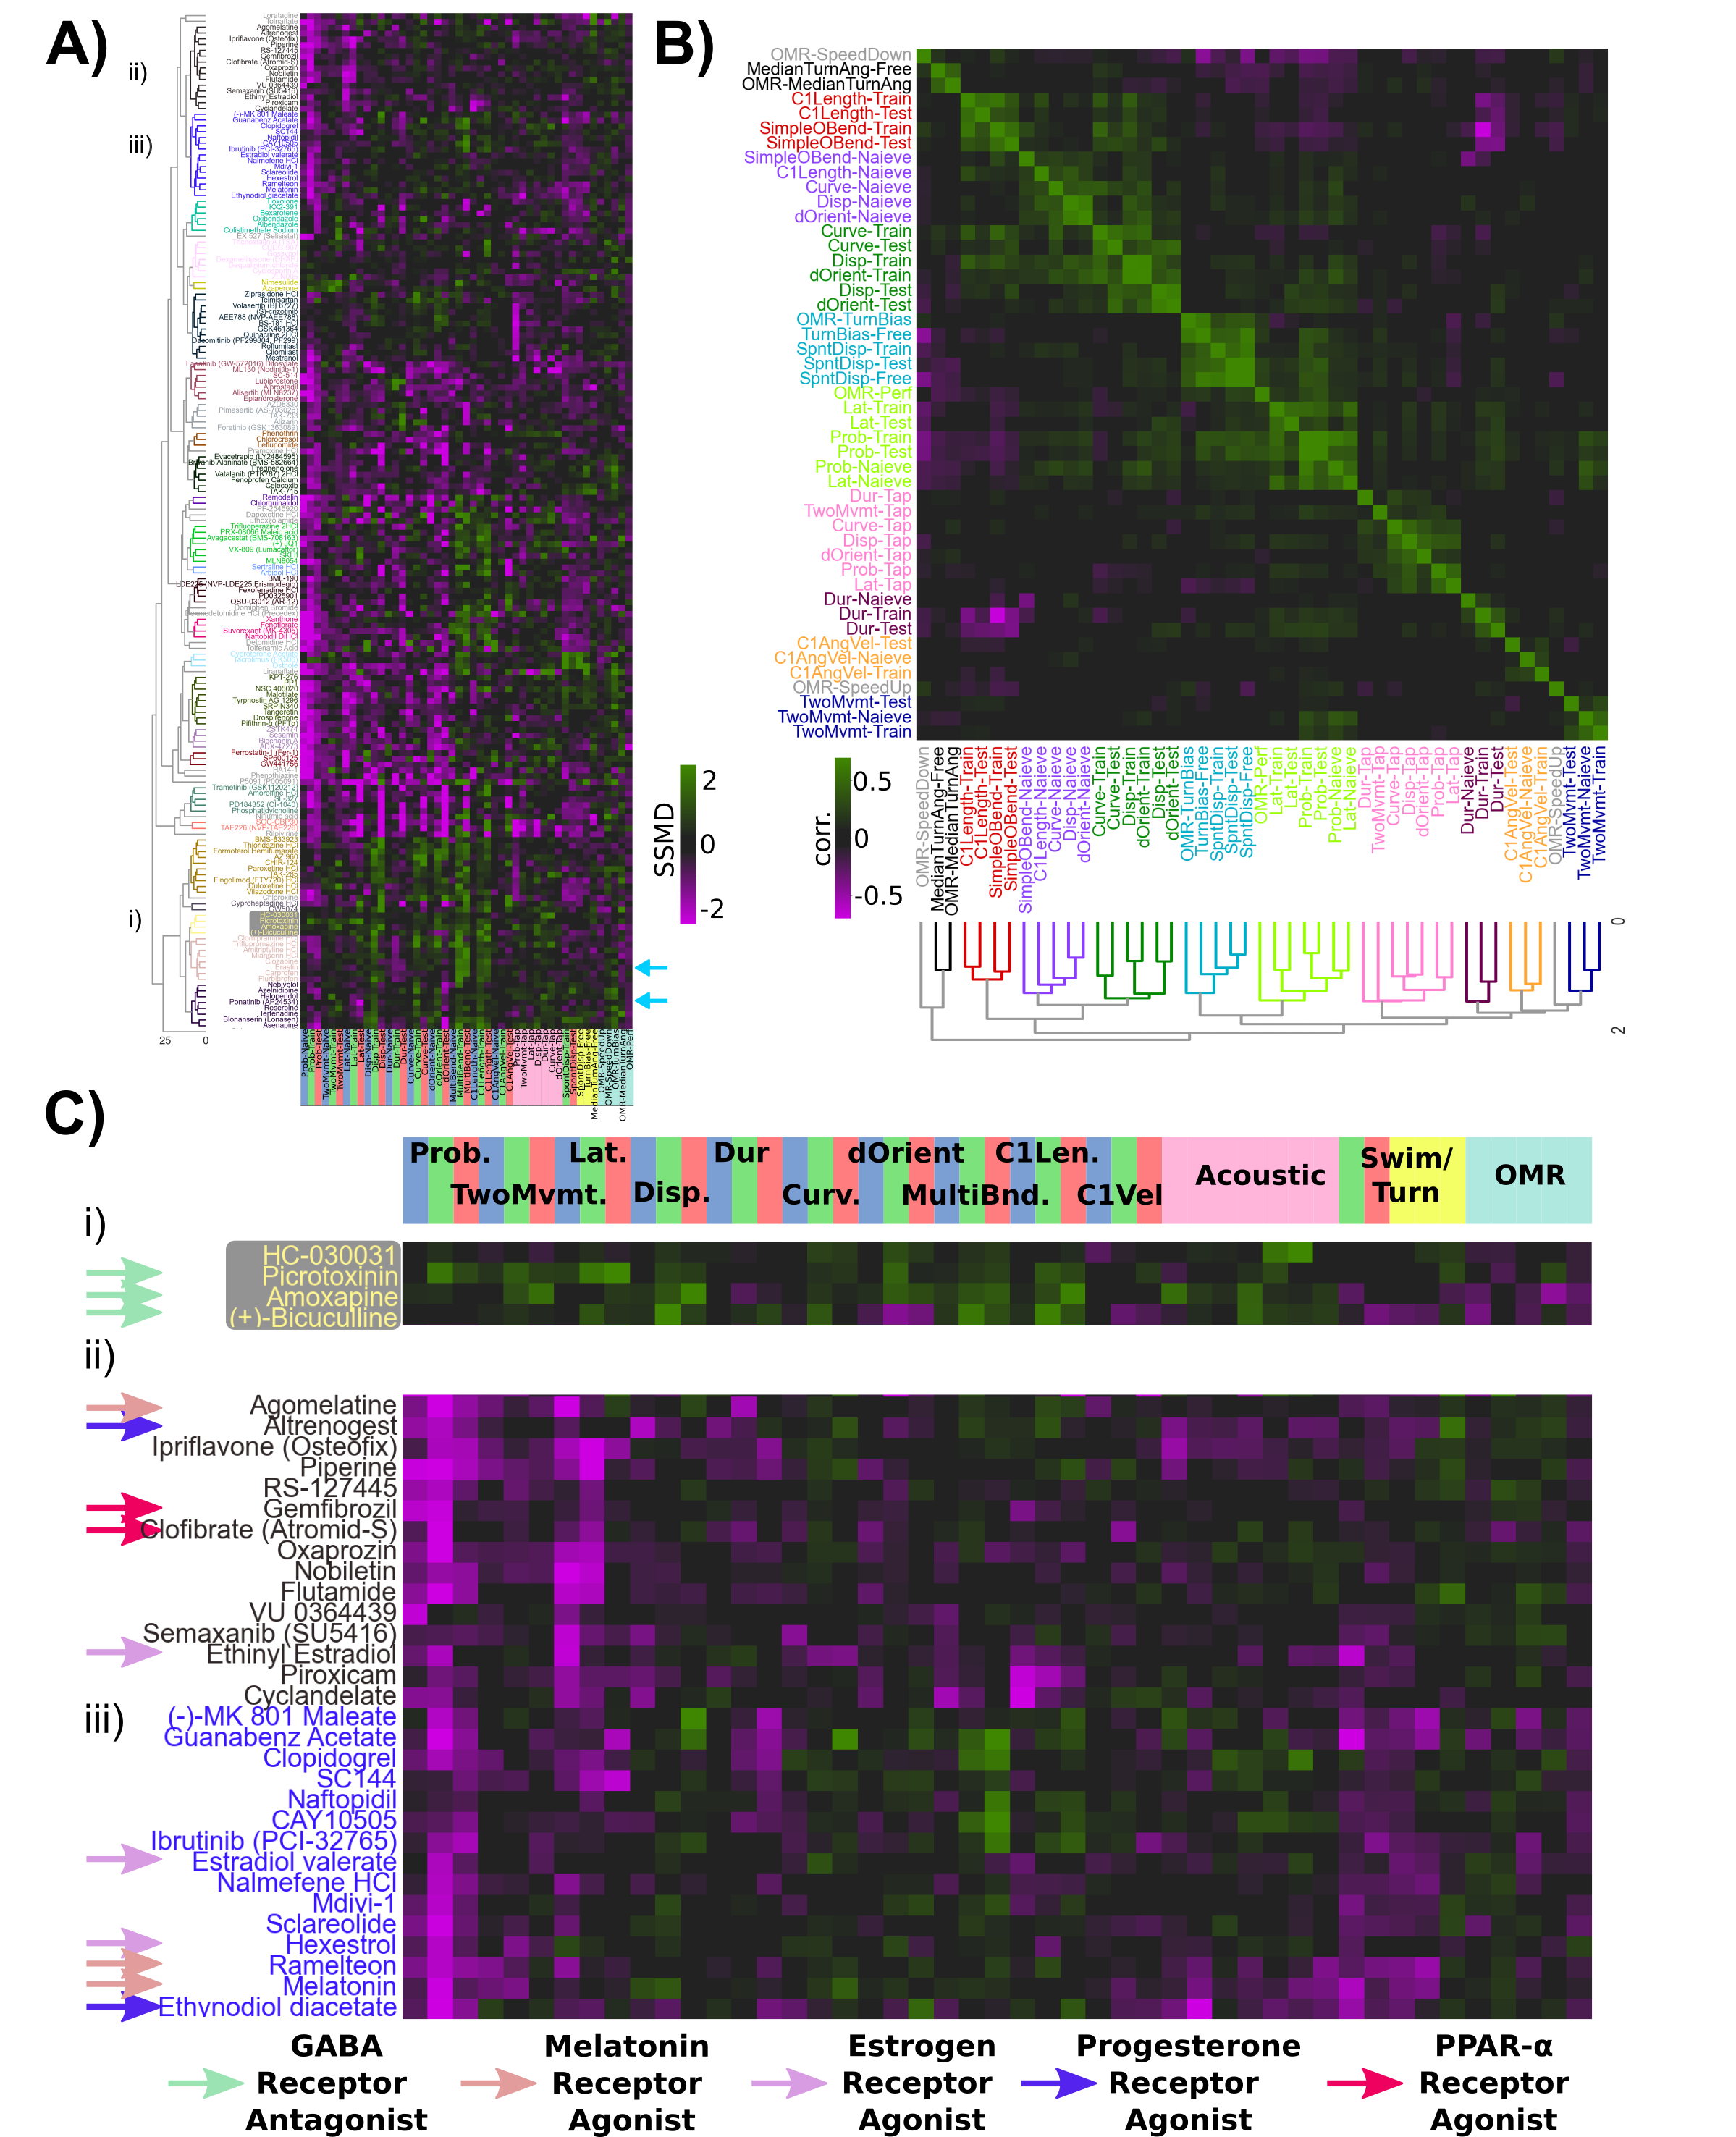
\includegraphics[width=0.87\linewidth]{Figure_2-ClusterFigure.png}
\caption{
Pharmaco-behavioural analyses of behaviour-modifying compounds. 
\textbf{A)} Clustered heatmap of the behavioural Fingerprints for the 176 hits of the screen, showing at least one behaviour measure with $ |SSMD| \geq 2 $. Clustering distance = ward, standardized euclidean. This led to the re-identification of Haloperidol and Clozapine as habituation modifiers (light blue arrows). 
\textbf{B)} Clustered correlogram of the Pearson correlation coefficients for the different measured components of behaviour across hits (same data as (A)) revealing the independence or co-modulation of behaviours. Clustering distance = average, correlation. 
\textbf{C)} Subsets of clustered heatmap from (A), highlighting the similar phenotypes exhibited by i) GABA Receptor antagonists and ii), iii) Melatonin receptor agonists, Estrogen receptor agonists, Progesterone receptor agonists and peroxisome proliferator-activated receptor alpha (PPAR$\alpha$) agonists. 
}
\label{fig:2}
\end{center}
\end{fullwidth}
\end{figure}

We screened a total of 1953 small molecule compounds for their acute effects on behaviour (\autoref{fig:1}-\autoref{table:1})), focusing on both activators and  inhibitors  with annotated targets. We were able to collect the full behavioural record of 1761 compounds  (\autoref{fig:1}D, \autoref{fig:1}-\autoref{table:2})), indicating that the fish survived the treatment and maintained their ability to swim. Using a threshold of \(\pm 2 \mathit{SSMD}\), we found that 176 drugs significantly altered at least one aspect of measured behaviour, yielding a 9\% hit rate. While the average effect was to suppress behavioural output \(\overline S \overline S \overline M \overline D = -0.20\), which could reflect non-specific toxicity or a generalized inhibition of motor output, the effect of most small molecules  induced both positive and negative changes in behavioural output, indicating that toxicity is not the primary phenotypic driver (\autoref{fig:2}A). While the false negative rate is difficult to determine since so little is known about the pharmacology of our system, we note that of the three small molecules we previously established to alter dark flash habituation that were included in the screen (Clozapine, Haloperidol and Pimozide), two were identified among our hits. 

To explore the pharmaco-behavioural space in our dataset we clustered small molecules  based on their behavioural phenotypes (\autoref{fig:2}A). This strategy can identify drugs that share common pharmacological targets, or perhaps distinct pharmacological targets that result in convergent behavioural effects \cite{Bruni2016-nq, Rihel2010-pj}. Indeed, drugs known to target the same molecular pathways often showed similar behavioural fingerprints lying proximal on the linkage tree, indicating that our dataset contains sufficient signal-to-noise to recover consistent pharmaco-behaviour relationships. 

Alternatively, drugs can be considered  as tools to manipulate different aspects of brain function agnostic to their molecular mechanisms. Consequently,  using similarities and differences among the induced alterations should uncover molecular and neural linkages among different behavioural outputs. Following this logic, the ability of a drug to co-modify different aspects of behaviour would reflect molecular and/or circuit-level dependencies. For example, visual behaviours that all depend upon the retinal photoreceptors should be similarly affected by any drugs that modulate phototransduction in these photoreceptors. We quantified these relationships by calculating the correlated effects on our different behavioural measurements across drugs (\autoref{fig:2}B). 

Consistent with our previous results highlighting uncorrelated learning across the behavioural components of the O-bend response during habituation \cite{Randlett2019-fi}, we found that different aspects of the response were independently affected pharmacologically, resulting in distinctive correlated groupings within the correlogram. While we previously found that O-Bend response Probability and Latency habituate independently in individual fish \cite{Randlett2019-fi}, in our drug screen data these appear to be tightly coupled (\autoref{fig:2}B, green cluster). This may result from their reliance on a common molecular-level mechanism that occurs in distinct circuit loci. However, the performance of the animals in the OMR assay under different treatments was also associated with O-bend Probability and Latency, suggesting that pharmacological modulation of general visual acuity could drive these correlations within the drug screen dataset.

These analyses confirm habituation behaviour manifests from multiple distinct molecular mechanisms that independently modulate different behavioural outputs. Our screen was successful in identifying small molecules that differentially modulate these distinct aspects of habituation behaviour, as well as acoustic, optomotor, and spontaneous behaviour. 

\subsection{Molecular pathways implicated in habituation}

For the remainder of the analyses we chose to focus on the mechanisms leading to the habituation of response probability, as this is the criterion for which it is easiest to identify the link between neural activity and behavior, providing the best entry point for studying the circuit mechanisms of long-term habituation. To identify the most promising hits, we sought to identify drugs that:

\begin{enumerate}
\item Have minimal effects on the naive response to DFs, but strong effects during the training and/or memory-retention periods. This would prioritize pathways that affect habituation, rather than simply DF responsiveness.

\item Have minimal effects on other aspects of behaviour. We purposefully assayed additional behaviours after habituation training in order to exclude compounds that would alter generalized arousal, movement ability/paralysis, or visual impairment. Such drugs would strongly influence DF responsiveness, but likely independently of pathways related to habituation. 

\item Show similar behavioural effects to other drugs screened that target the same molecular pathway. Such relationships can be used to cross validate, yet we note that our library choice was very broad, and target coverage is non-uniform. Therefore a lack of multiple hits targeting the same pathway should not necessarily be taken as strong evidence of a false positive. 
\end{enumerate}

\begin{figure}
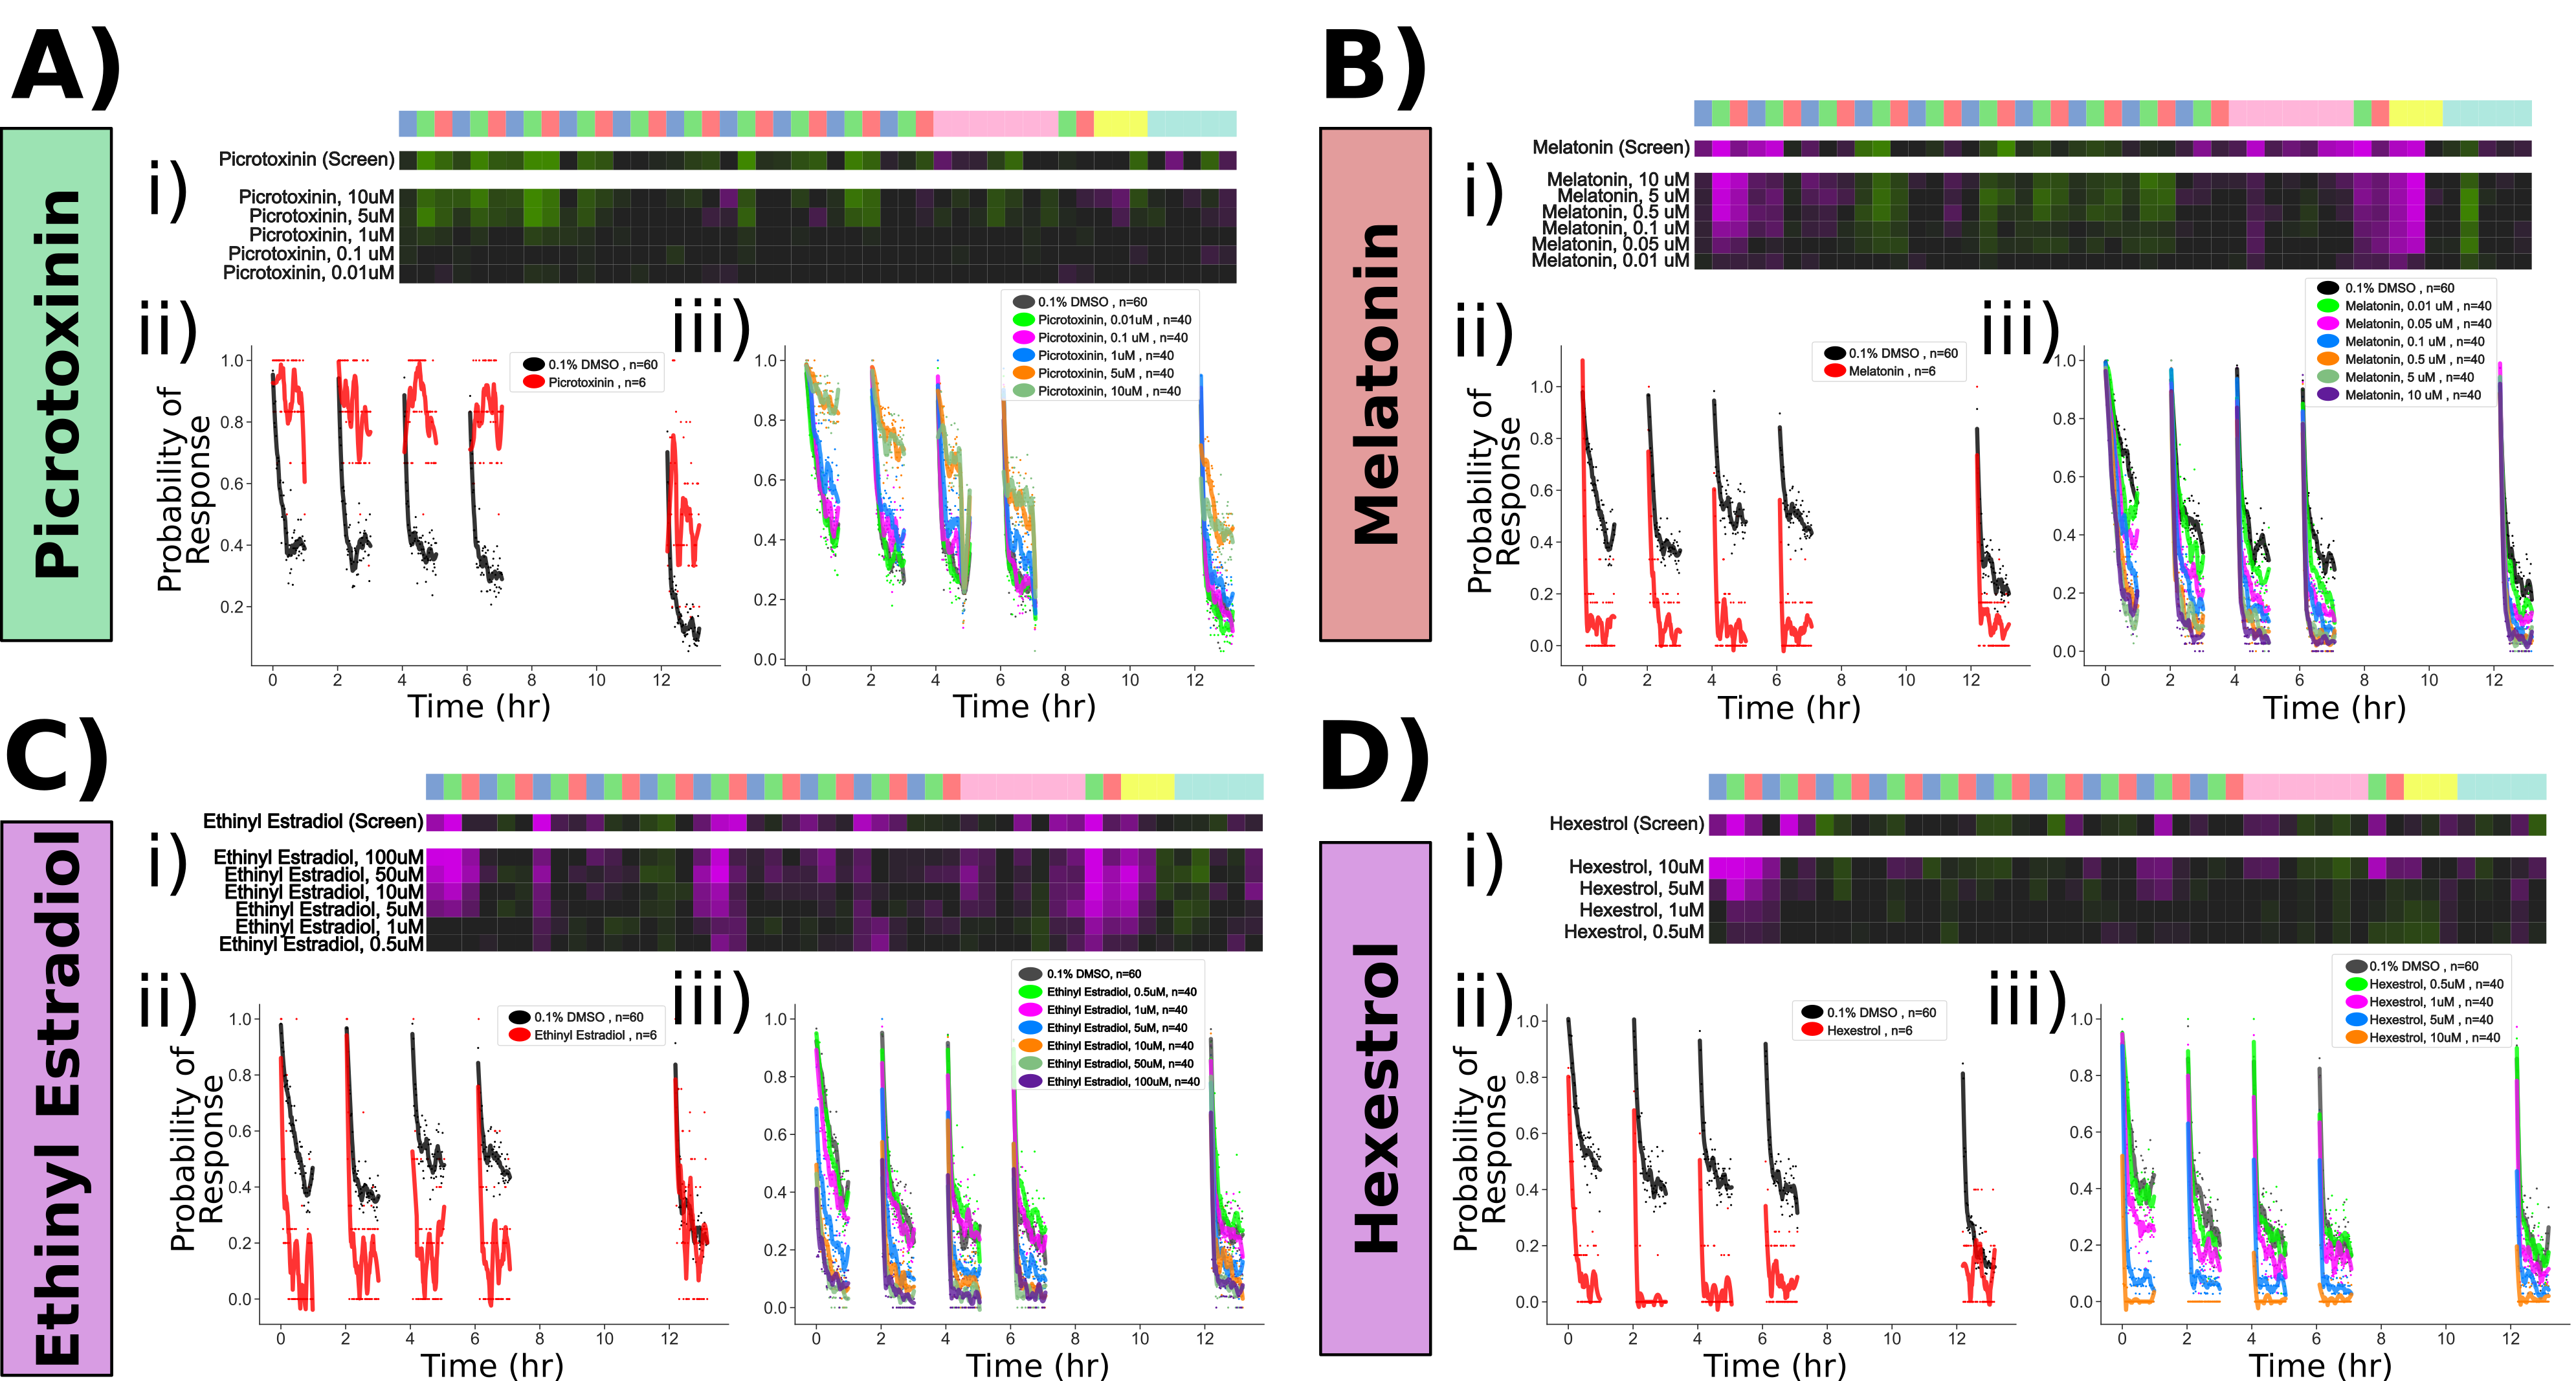
\includegraphics[width=0.9\textwidth]{Figure_3-HitsValidation.png}

\caption{
Confirmed pharmacological modulators of habituation
Dose response studies for \textbf{A)} Picrotoxinin, \textbf{B)} Melatonin, \textbf{C)} Ethinyl Estradiol and \textbf{D)} Hexestrol. Displayed for each treatment are: 
i) Behavioural fingerprint for the original screen data (10 uM), and the dose response data.
ii) Original screen data for the probability of response to DF stimuli. Each dot is the probability of response to one flash. Lines are smoothed in time with a Savgolay Filter (window = 15 stimuli, order=2).
iii) Dose response data for the probability of response, plotted as in ii)
}
\label{fig:3}
\figsupp[Pharmacological manipulation of control behaviours and response displacement during habituation]
{Pharmacological manipulation of control behaviours and response displacement during habituation.
Dose response studies for \textbf{A)} Picrotoxinin, \textbf{B)} Melatonin, \textbf{C)} Ethinyl Estradiol and \textbf{D)} Hexestrol. Displayed for each treatment are: 
i) Violin plots for the dose response data, showing the probability of response to 30 acoustic tap stimuli. Horizontal lines = individual fish.
ii) Violin plots for the dose response data OMR performance. Horizontal lines = individual fish. Statistical tests: Mann Whitney with bonferroni correction, ns=not significant; $p \leq ****=1x10^{-4}; ***=1x10^{-3}; **=1x10^{-2}; *=0.05$. 
\textbf{E)} Treatment with Picrotoxinin inhibits the decreases in movement displacement during habituation training. 
\textbf{F)} Treatment with Melatonin inhibits the decreases in movement displacement during habituation training. Each dot is the mean response of the population to one flash. Lines are smoothed in time with a Savgolay Filter (window = 15 stimuli, order=2).}{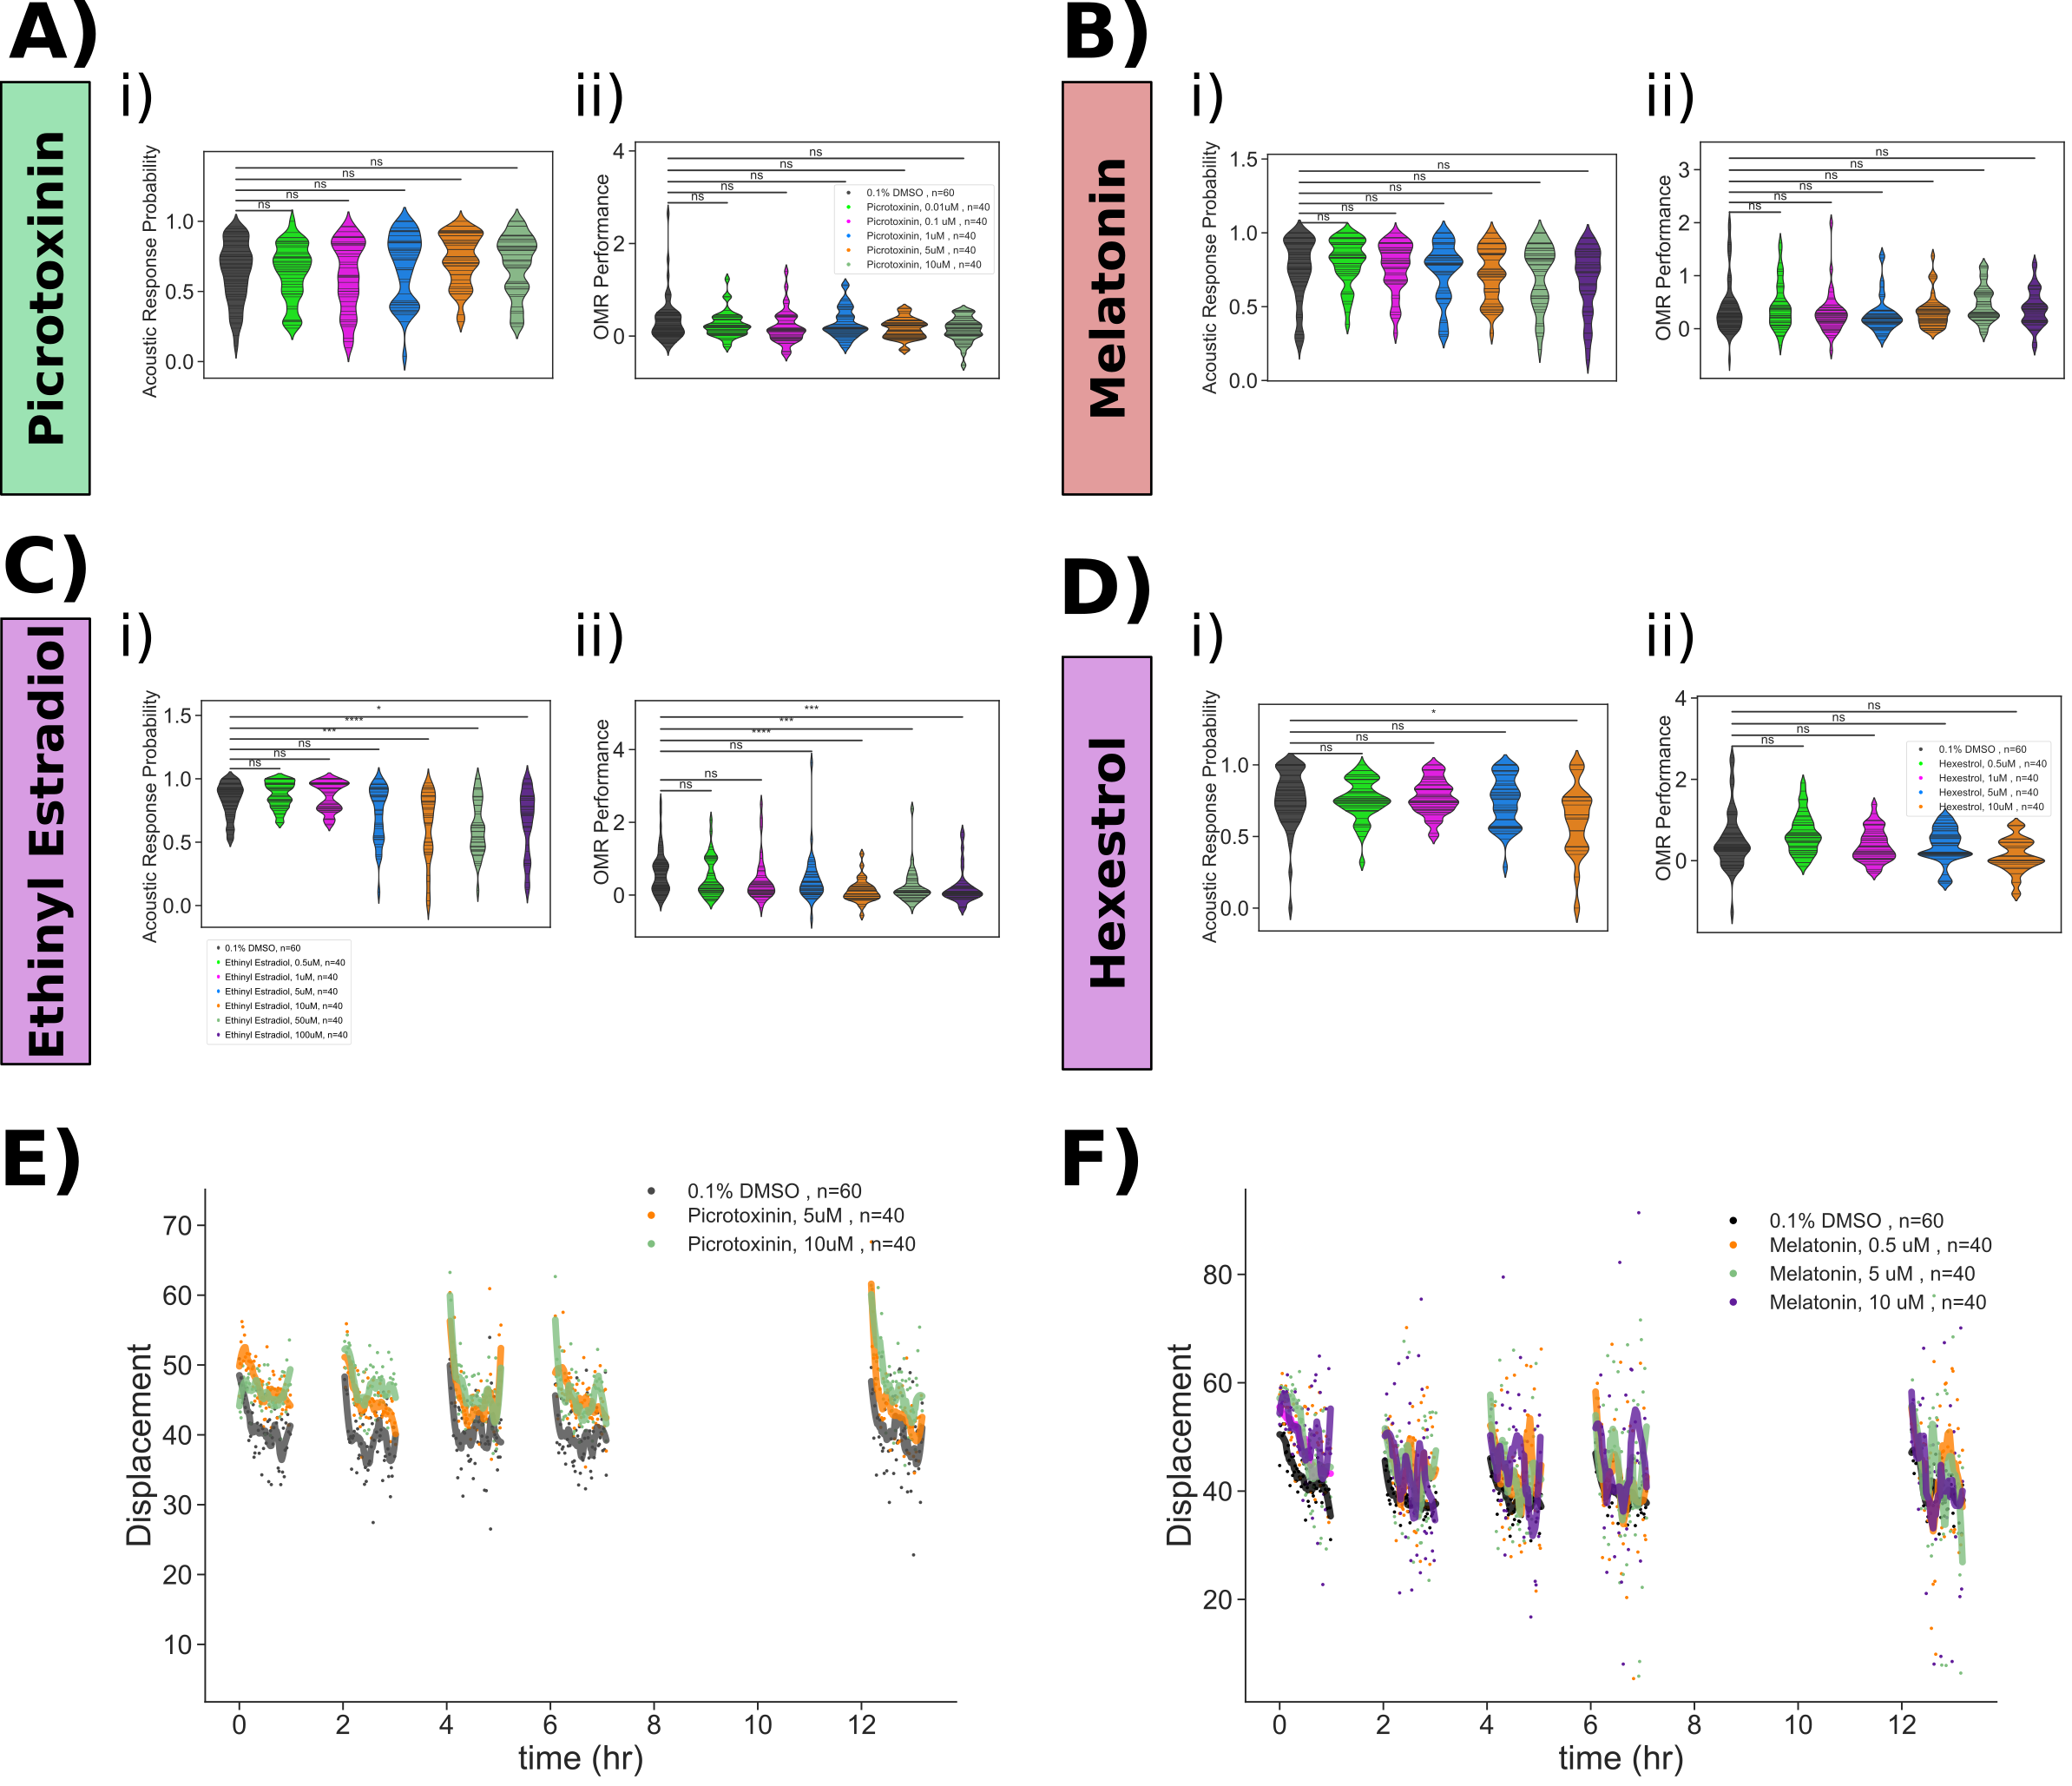
\includegraphics[width=14cm]{FigureS1_DrugBehavData_wDisp}}
\label{fig:S3}
\end{figure}


This prioritization led us first to the identification of the GABA\textsubscript{A/C} Receptor antagonists Bicuculline, Amoxapine, and Picrotoxinin (PTX). PTX treatment had the strongest effects, with increased responsiveness to DFs during the training and test periods, indicative of defects in habituation (\autoref{fig:2}Ci). Dose-response experiments confirmed a strong effect of PTX on inhibiting the progressive decrease in responsiveness during habituation learning at 1-10uM doses. Importantly, like the naive dark-flash response, the acoustic and optomotor response were not inhibited (\autoref{fig:3}A, \autoref{fig:3}-\autoref{fig:S3}1A). While strong GABA\textsubscript{A/C}R inhibition will result in epileptic activity in larval zebrafish, we did not observe evidence of seizure-like behaviour at these doses, consistent with previous results (Bandara et al., 2020). Therefore, we conclude that partial antagonism of GABA\textsubscript{A}R and/or GABA\textsubscript{C}R is sufficient to strongly suppress habituation, indicating that GABA plays a very prominent role in habituation resulting in this strong sensitivity to manipulation. This is consistent with a model in which the potentiation of inhibition actively silences sensory-induced activity during habituation to suppress motor output, rather than the depression of excitatory neurotransmission in the activated pathway \cite{Cooke2020-mz, Ramaswami2014-du}. 

We next turned our attention to the upper portion of the clustered behavioural fingerprint graph (\autoref{fig:2}A), where strong and relatively specific inhibition of responsiveness during training and testing were observed, indicative of enhanced habituation (\autoref{fig:2}Cii, iii). Among the hits observed here were multiple agonists of both Melatonin and Estrogen receptors, indicating that neuro-hormonal signaling may play a prominent role in plasticity underlying habituation. Dose response studies with Melatonin confirmed strong potentiation of habituation (\autoref{fig:3}B). Melatonin did cause a decrease in spontaneous movement behaviour, consistent with its role in arousal/sleep regulation in zebrafish and other vertebrates \cite{Gandhi2015-vw, Zhdanova2001-dq}, yet Melatonin did not inhibit the naive response to dark flashes, the responsiveness to acoustic stimuli or OMR performance (\autoref{fig:3}B, \autoref{fig:3}-\autoref{fig:S3}1A)1B), indicating it does not cause generalized sedation but modulates specific aspects of behaviour at these doses, including increasing habituation. 

We similarly validated that the Estrogen Receptor agonists Ethinyl Estradiol and Hexestrol, potentiated habituation at 5-100uM and 1-10uM doses, respectively (\autoref{fig:3}C,D). However, Ethinyl Estradiol strongly suppressed movement rates at these doses, and both treatments suppressed acoustic responsiveness and OMR performance at doses >=10uM (\autoref{fig:S3}1C,D). Therefore, it is less clear how specific or generalized Estrogen Receptor agonism is on behaviour, although the effective doses of Hexestrol for influencing habituation (1-5uM) were lower than those that significantly affected other behaviours (10uM). Nevertheless we decided to focus on PTX and Melatonin for the remaining experiments. 


Our screening approach has identified both expected (GABA) and unexpected (Melatonin, Estrogen) pathways that strongly modulate habituation of responsiveness. We have also implicated multiple additional pathways in habituation, including Progesterone and PPAR$/alpha$ (\autoref{fig:2}C), as well as OMR, acoustic and spontaneous behaviour, which can be mined for future projects investigating the molecular basis of behaviour. 

\subsection{Dark flash-induced neural activity is broadly inhibited during habituation}


\begin{figure}
\begin{fullwidth}
\begin{center}
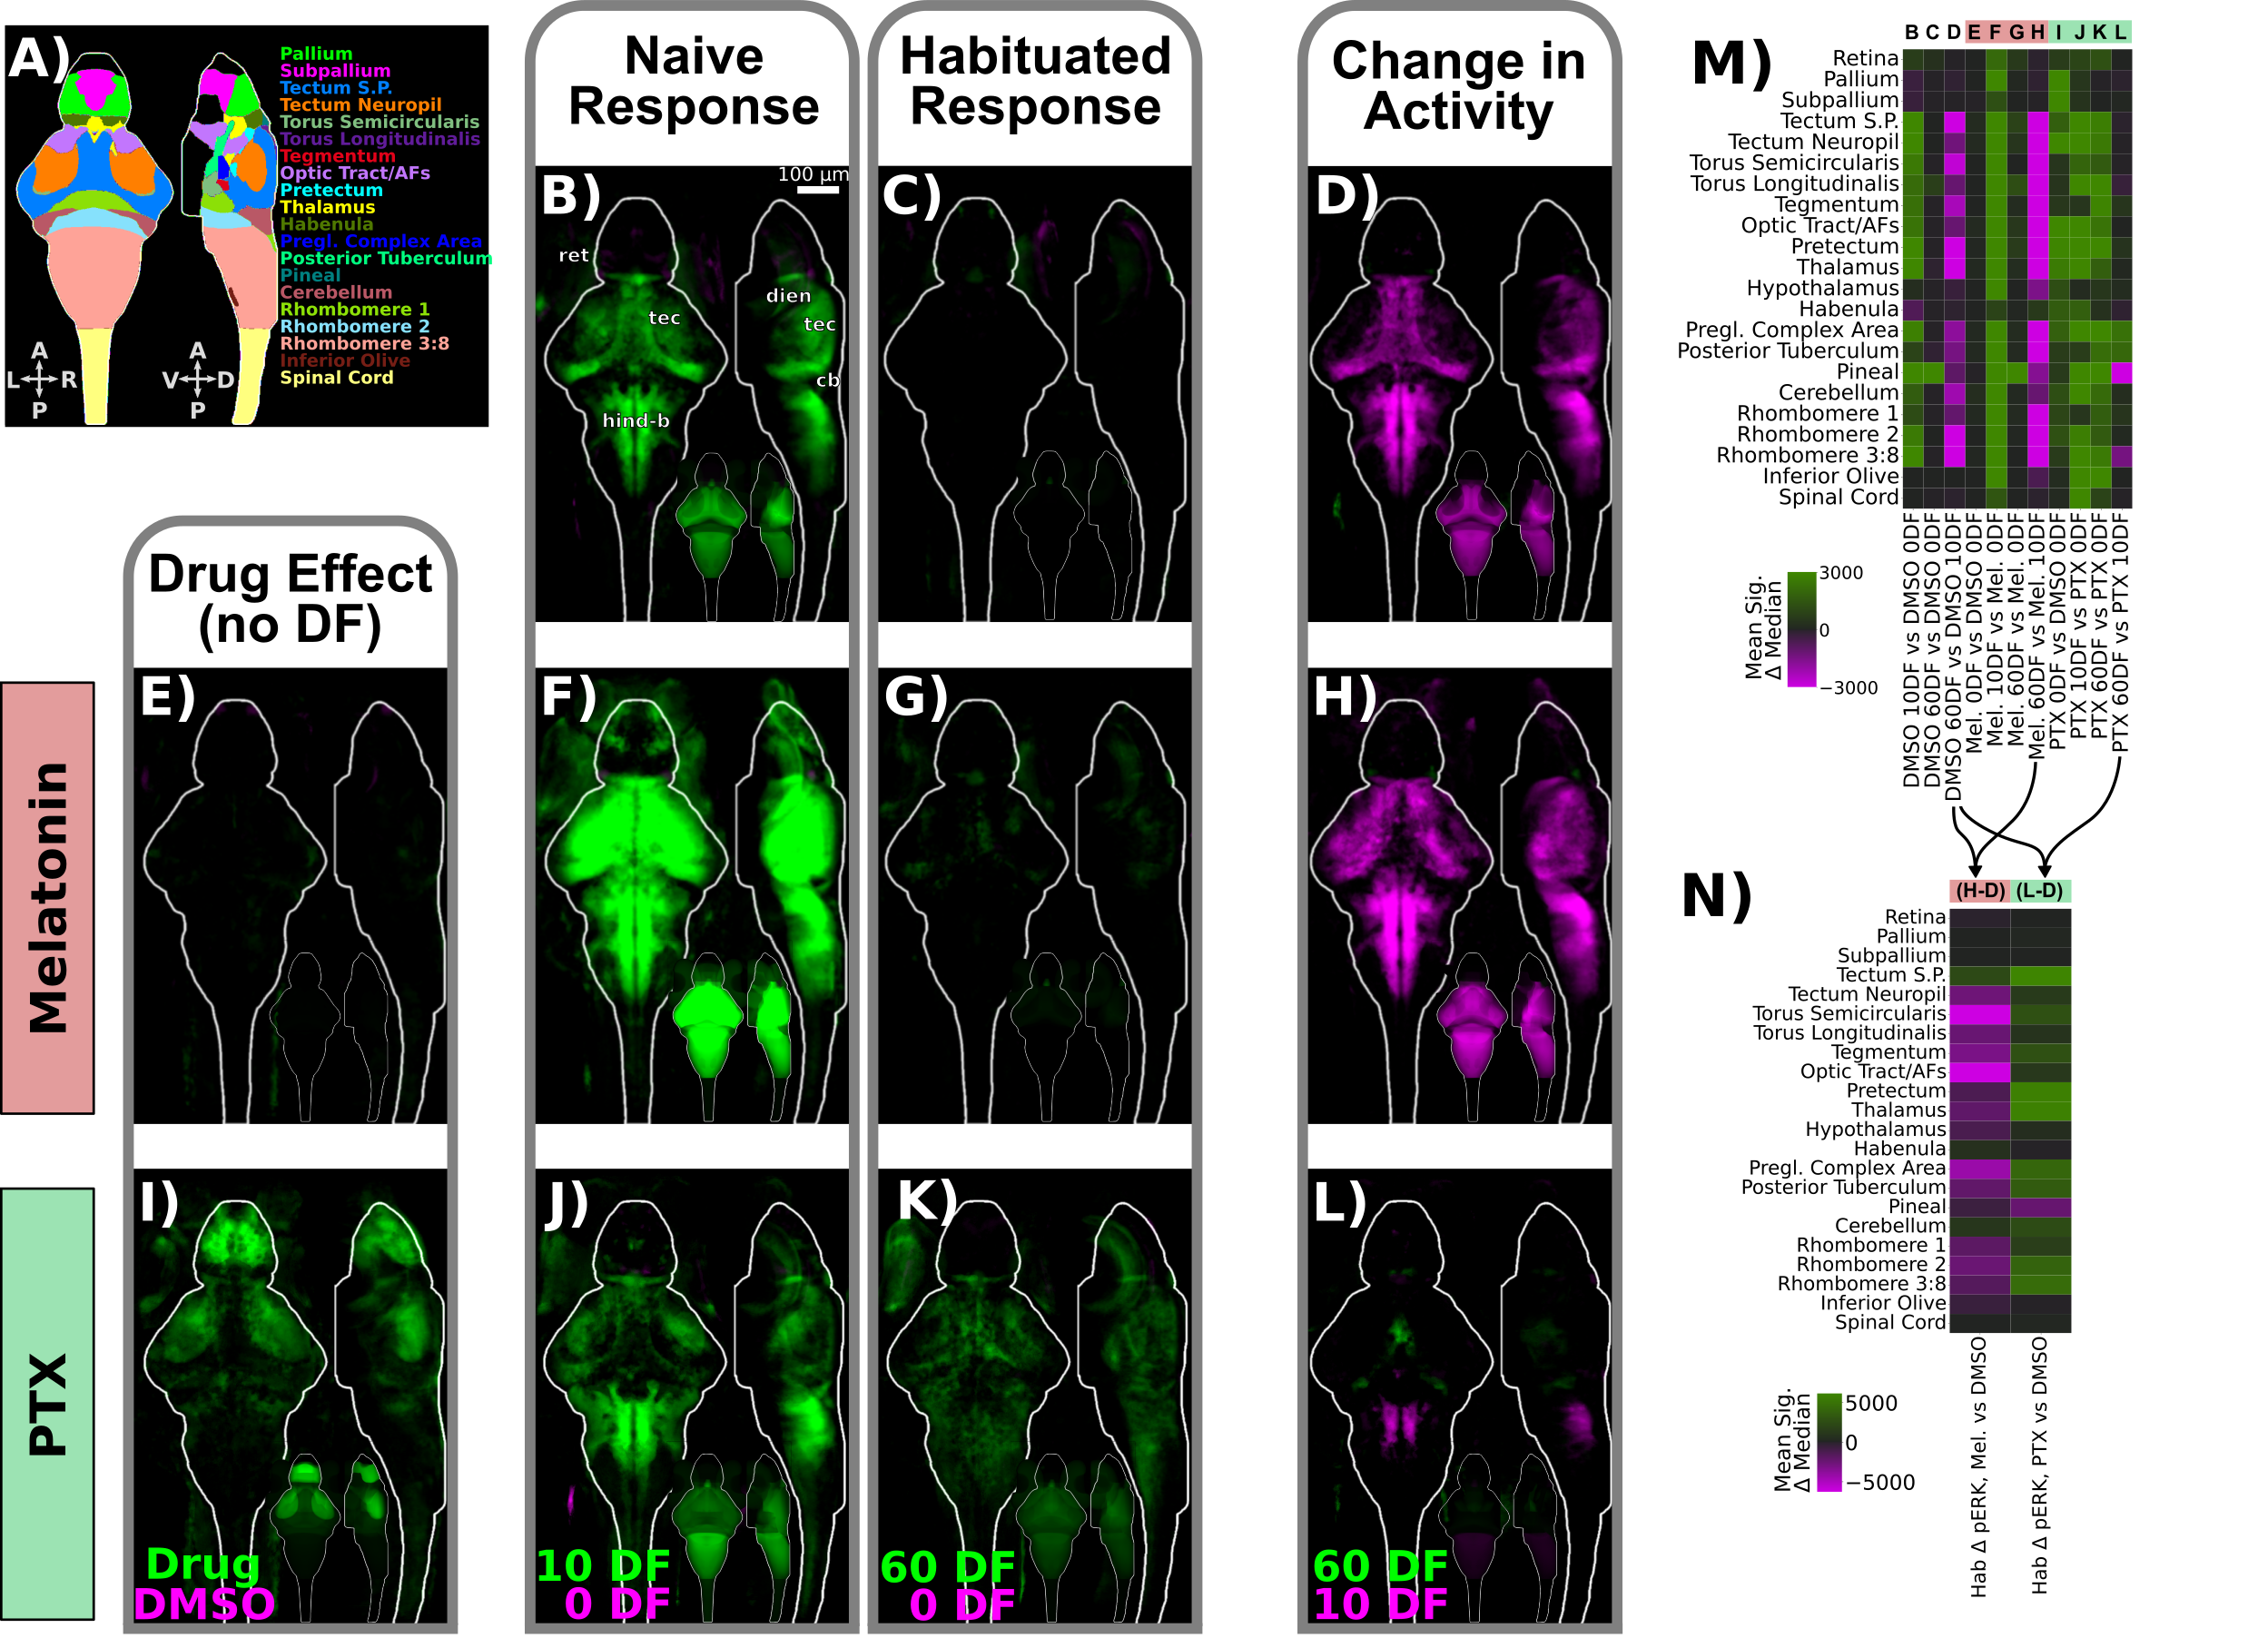
\includegraphics[width=0.93\linewidth]{Figure4-pERKResults.png}
\caption{
pERK-based whole-brain mapping of altered neural activity during habituation
\textbf{A)} Anatomical regions in the Z-Brain coordinate space used for image display and analyses. A = anterior, P = posterior, L = left, R = right, V = ventral, D = dorsal. 
\textbf{B-L)} MAP-Maps showing areas with whole-brain differences in pERK/tERK staining intensity, with green and magenta representing significantly increased staining in the relevant group in the pairwise comparison. Shown as summed intensity projections in the Z-Brain coordinate space in the dorso-ventral (left) and sagittal (right) dimensions. Lower inset represents the average signal binned by brain regions. MAP-Maps were calculated for pairwise differences between the following treatments in:
Column 1: “Drug Effect (no DF)” = drug treatment with no stimulation (green) vs. DMSO with no DFs (magenta)
Column 2: “Naive Response” = Response to 10 DFs (green) vs. 0 DFs (magenta)
Column 3: “Habituated Response” = Response to 60 DFs (green) vs. 0 DFs (magenta)
Column 4:  “Change in Activity” = Response to 60 DFs (green) vs. 10 DFs (magenta). 
Pharmacological treatments arranged in rows as: 
Row 1) 0.1% DMSO
Row 2) Melatonin, 0.1uM in 0.1% DMSO
Row 3)  Picrotoxinin (PTX), 5uM in 0.1% DMSO. 
ret = retina, dien = diencephalon, tec = tectum, cb = cerebellum, hind-b = hindbrain
\textbf{M)} Mean signal in brain regions for each of the experiments shown in A-K, shown as a vector in the heatmap. Same data as insets in A-K
\textbf{N)} Difference in the MAP-Map signals in brain areas comparing drug treated fish to DMSO control when stimulated with 60 DF vs 10 DF. Resultant differences reflect altered activity during habituation training by the drug treatment. 
Number of imaged fish per experimental group were: 0.1\% DMSO, 0 DF = 26; 0.1\% DMSO, 10 DF = 29; 0.1\% DMSO, 60 DF = 23; Melatonin, 0 DF = 29; Melatonin, 10 DF = 23; Melatonin, 60 DF = 19; Picrotoxinin, 0 DF = 28; Picrotoxinin, 10 DF = 23; Picrotoxinin, 60 DF = 27.
DF = Dark Flash, Mel = Melatonin, PTX = Picrotoxinin. }
\label{fig:4}
\end{center}
\end{fullwidth}
\end{figure}

Having identified molecular components of habituation, we next aimed to identify how these molecules act within the circuit to modify neural activity and subsequent behavioural output. For this we used the MAP-Mapping strategy, which allows us to measure whole-brain activity patterns from freely-swimming larvae based on their relative levels of pERK immunostaining \cite{Randlett2015-hy}. MAP-Mapping yields a picture of the activity patterns in the experimental setting that is closest to the drug-screen situation. We determined which areas of the brain respond to DFs by comparing the pERK patterns in larvae stimulated with 10 DFs at 1 min intervals, to those that were not stimulated (\autoref{fig:4}B, M). These larvae were treated with 0.1\% DMSO as a vehicle control for the pharmacological experiments (below). This revealed widespread activation of the brain in response to DFs, including visual areas such as the retina (ret), tectum (tec), pineal, petecum and thalamus, indicating that a distributed sensory circuit is activated by DFs. However, relatively little signal was observed in the telencephalon or the habenula, indicating that these structures are not central to the DF response. Strong activation was seen in the hindbrain and cerebellum, likely reflecting motor-related signals related to the O-bend response. 

We then asked how this pattern changes as the animals learn. We focused on a single training block of 60 DFs, as this is the period under which the strongest learning takes place, and where our chosen pharmacological treatments have the strongest effects relative to controls (\autoref{fig:3}). Since the pERK indicator integrates over the last ~15 minutes of life, but is biased towards the terminal 5 minutes \cite{Randlett2015-hy}, these experiments were designed to highlight the final DFs after learning has taken place.



Indeed, these larvae showed much weaker activation across most of the brain (\autoref{fig:4}C, M), which resulted in widespread decreases in neural activity compared to the 10 DF group (\autoref{fig:4}D, M). This indicates that the plasticity underlying habitation affects neurons relatively early in the visual pathway, resulting in depressed activation in primary sensory areas (e.g. tectum and pretectum), as well as motor-related areas presumed to lie more downstream in the sensory-motor circuit (e.g. tegmentum and hindbrain). However, the retina was not depressed, indicating that habituation occurs downstream of this sensory ganglion. 

To test our model of early visual pathway plasticity, we asked if the inhibition of habituation (via GABA\textsubscript{A/C}R inhibition using PTX), or its potentiation (via Melatonin), led to the expected alterations in MAP-Maps. We first determined that Melatonin alone failed to strongly alter neural activity (\autoref{fig:4}E, M), while PTX induced the expected activation associated with GABA inhibition, most prominently in the telencephalon (\autoref{fig:4}I,M). Surprisingly, the naive response to DFs was potentiated in the Melatonin treatment and suppressed in the PTX treatment relative to their baseline activity, indicating that alterations in naive visual acuity for DFs is insufficient to explain the habituation phenotypes associated with these treatments (\autoref{fig:4}F,J,M). Finally, when assaying for the depression of activity in trained fish relative to their naive response to DFs, we found that Melatonin treatment did indeed increase the observed depression, while PTX inhibited this depression, including in primary visual areas proximal to the retinal arborisation fields, the thalamus, pretectum, hypothalamus, and tectum neuropil (\autoref{fig:4}G,H,K-N). 

These whole-brain functional activity surveys demonstrate that habituation learning is associated with a surprisingly strong depression of neural activity, considering that at the behavioural level larvae remain quite responsive to DF stimuli after only one training block (Figure 1-3). These apparent discrepancies may reflect the presumably complex and non-linear relationship between neural activity and pERK responsiveness. Combined with the pharmacological manipulations, these experiments support a model in which habituation plasticity begins early in the visual pathway. However, the temporal and spatial resolution of these experiments is insufficient to differentiate how individual neurons adapt during habituation, and therefore do not exclude the possibility that habituation occurs within the the retina, perhaps at the retinal ganglion cell terminals, where the central brain would simply receive an increasingly depressed signal from the periphery. 

\subsection{Volumetric 2-photon Ca\textsuperscript{2+} imaging of habituation learning}

\begin{figure}
\begin{fullwidth}
\begin{center}
\includegraphics[width=0.9\linewidth]{Figure5 - Ca2Imaging.png}
\caption{
Volumetric 2-photon Ca\textsuperscript{2+} imaging of dark flash habituation
\textbf{A)} \textit{Tg(elavl3:H2B-GCaMP7f)} larvae were imaged across 12 z-planes at 10um steps. ROIs segmented using suite2p \cite{Pachitariu2017-ad} are overlaid in random colors. 
\textbf{B)} Density of detected ROIs registered and plotted in the Z-Brain coordinate space. n=1,050,273 ROIs across 34 larvae. 
\textbf{C)} Cropped field of view used for plotting Ca\textsuperscript{2+} imaging data and approximate anatomical localizations of major brain areas: dien=diencephalon, mid-b = midbrain, cb = cerebellum, hind-b = hindbrain, io = inferior olive, ret = retina, tec = tectum
\textbf{D)} Functional responses of the population of neurons in the same fish as A), plotted as a clustered heatmap (“rastermap” \cite{Pachitariu2017-ad}, \href{https://github.com/MouseLand/rastermap}{github.com/MouseLand/rastermap}), where rows represent individual neurons ordered by the similarities in their activity. Darker shades reflect increased activity. This clustering reveals neurons that are tuned to the DF stimuli (pink box) or motor events (green box). Dashed trace above the heatmap depicts the DF stimulus convolved with a kernel approximating H2B-GCaMP7f kinetics.
\textbf{E)} ROIs in an individual fish plotted based on their correlation and tuning to regressors defining either Motor or DF stimulus events, highlighting the spatial distributions of these tunings across the imaged population. Plotted as a maximum intensity projection. 
\textbf{F)} Same analysis as E, but across the entire population of 34 larvae. 
\textbf{G)} ROIs in an individual fish plotted based on their correlation and tuning to regressors defining either the first or last three DF stimuli. 
\textbf{H)} Same analysis as G, but across the entire population of 34 larvae. tl = torus longitudinalis
}
\label{fig:5}
\figsupp[Validation of motion analysis based on image artifacts during 2-photon imaging]
{Validation of motion analysis based on image artifacts during 2-photon imaging
\textbf{A)} Motion indexes as calculated based on tail tracking (blue) and based on decreases in the correlation between individual frames and the reference frame used for motion alignment (orange) across the entire imaging experiment (65 minutes). 
\textbf{B)} Same analysis as (A), for a different larva. 
\textbf{C)} Cross-correlation plot comparing the two motion index vectors. Mean across 6 larvae, and line thickness = standard error. 
}{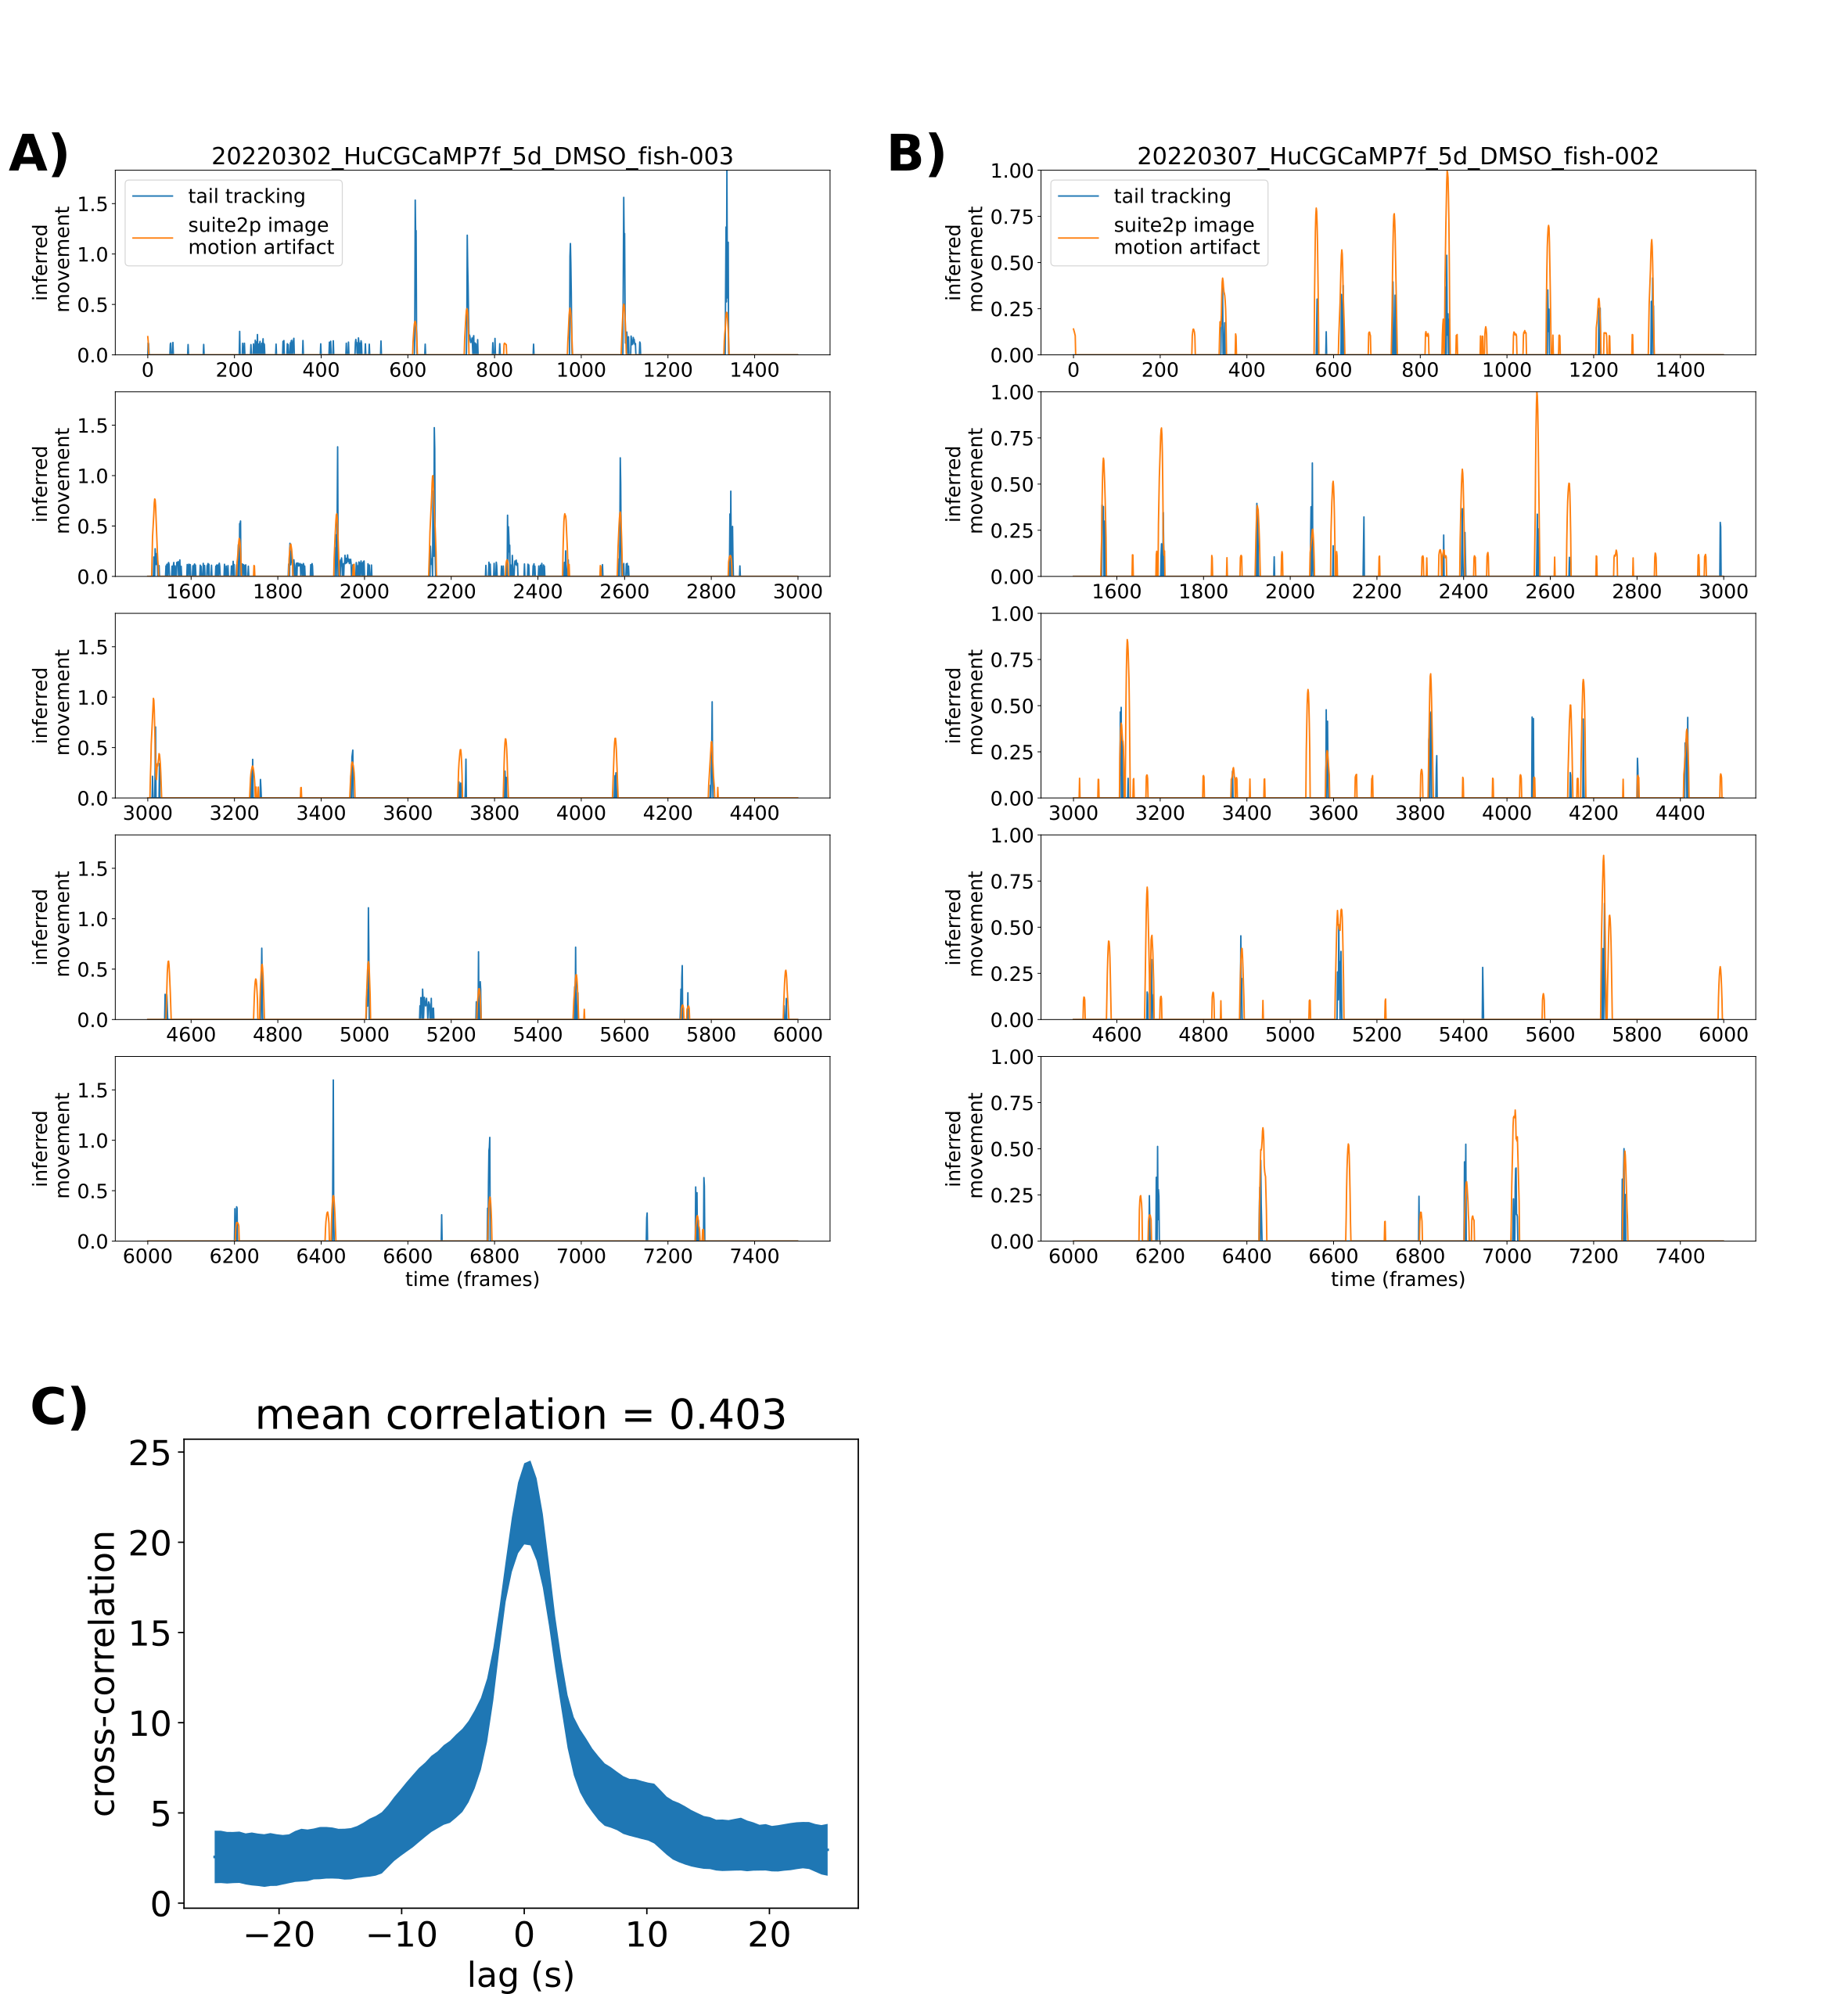
\includegraphics[width=14cm]{FigureS2_MotionAnalysis.png}}
\label{fig:S5}
\end{center}
\end{fullwidth}
\end{figure}

Having identified the regional alterations in activity associated with habituation learning, we next asked how the properties and individual neurons within the DF responsive circuit adapt during habituation. We used a head-fixed paradigm to perform 2-photon Ca\textsuperscript{2+} imaging during habituation learning. We expressed nuclear-targeted GCaMP7f pan-neuronally and imaged with a resonant scanner and piezo objective, enabling us to cover a volume of ~ 600 x 300 x 120 uM (x,y,z) sampled at 0.6 x 0.6 x 10 uM resolution, leading to the detection of 30890±3235 ROIs per larvae (±SD, \autoref{fig:5}A,C). ROIs were aligned to the Z-Brain atlas coordinates \cite{Randlett2015-hy}, demonstrating that this volume spans most of the areas implicated in DF habituation by our MAP-Mapping experiments (\autoref{fig:4}), including the majority of the midbrain, hindbrain, pretecum and thalamus (\autoref{fig:5}A-C). Visual stimuli were delivered via a red LED, and larvae were stimulated with 60 DFs at 1 min intervals to induce habituation learning. This induced strong Ca\textsuperscript{2+} activity in neurons (\autoref{fig:5}C), some of which were clearly associated with the DF stimuli. Ca\textsuperscript{2+} transients in response to DFs generally decreased across the 60 stimuli, though this pattern was not seen in all neurons, and substantial heterogeneity in their adaptations were observed. Strong correlated patterns were also seen in large groupings of neurons, predominantly in the hindbrain, which were associated with movement events through their correlation with motion artifacts in the imaging data (\autoref{fig:5}-\autoref{fig:S5}). 

To explore the spatial patterns in these datasets we used a 2-dimensional lookup table to simultaneously visualize the correlation and bias of Ca\textsuperscript{2+} fluctuations with regressors representing either DF stimuli or movement (\autoref{fig:5}E, F). This revealed segregated populations of neurons coding for the DFs (pink) and movement (green/teal). Similar patterns are visible in individuals and across the entire population of 34 larvae. As expected, DF-tuned neurons were located predominantly in visual sensory areas in the midbrain (tectum) and diencephalon (pretectum and thalamus). Motor-coding neurons dominated in the hindbrain, with the exception of the cerebellum and inferior olive, which was predominantly tuned to the sensory stimulus. Some neurons did show approximately equal correlation values to both stimuli, as evidenced by the blue-ish hues. Finally, some areas of the brain appeared to contain mixtures of neurons with different coding properties, including the ventral diencephalon and midbrain. 

To determine if there was any spatial logic to how different neurons adapt their responsiveness to DFs during imaging we plotted the ROIs using a lookup table highlighting the preference of ROIs for either the first three DFs (pink, naive response), or last three DFs (green, trained response). Strong preferences for the naive stimuli reflects a depressing response profile (\autoref{fig:5}G, H). Indeed, most neurons did show tunings consistent with strong depression, however there were neurons who showed an equal preference for naive and trained stimuli, or even stronger preference for the latter, indicating stable or potentiating response profiles. These potentiating neurons were mostly contained in the dorsal regions of the brain, including the torus longitudinalis, cerebellum and dorsal hindbrain. These results demonstrate that while the majority of neurons across the brain depress their responsiveness during habituation, a smaller population of neurons exists that show the opposite pattern. 

From these experiments we conclude that habituation does not occur exclusively within the retina, as in such a model neurons that show stable responses or that potentiate would not be present in the brain. Instead, these data are consistent with the model arising from our pERK analysis, where habituation begins early within the visual pathway, but downstream of the retina. However, the fact that non-depressing neurons are observed within structures like the caudal hindbrain and the cerebellum indicates that even in motor-related brain regions contain non-depressed signals, and thus plasticity could also be occurring in regions very downstream in the visual sensory-motor pathway.
\pagebreak
\subsection{Functional classification and anatomical localization of neuronal types observed during habituation learning}

\begin{figure}
\begin{fullwidth}
\begin{center}
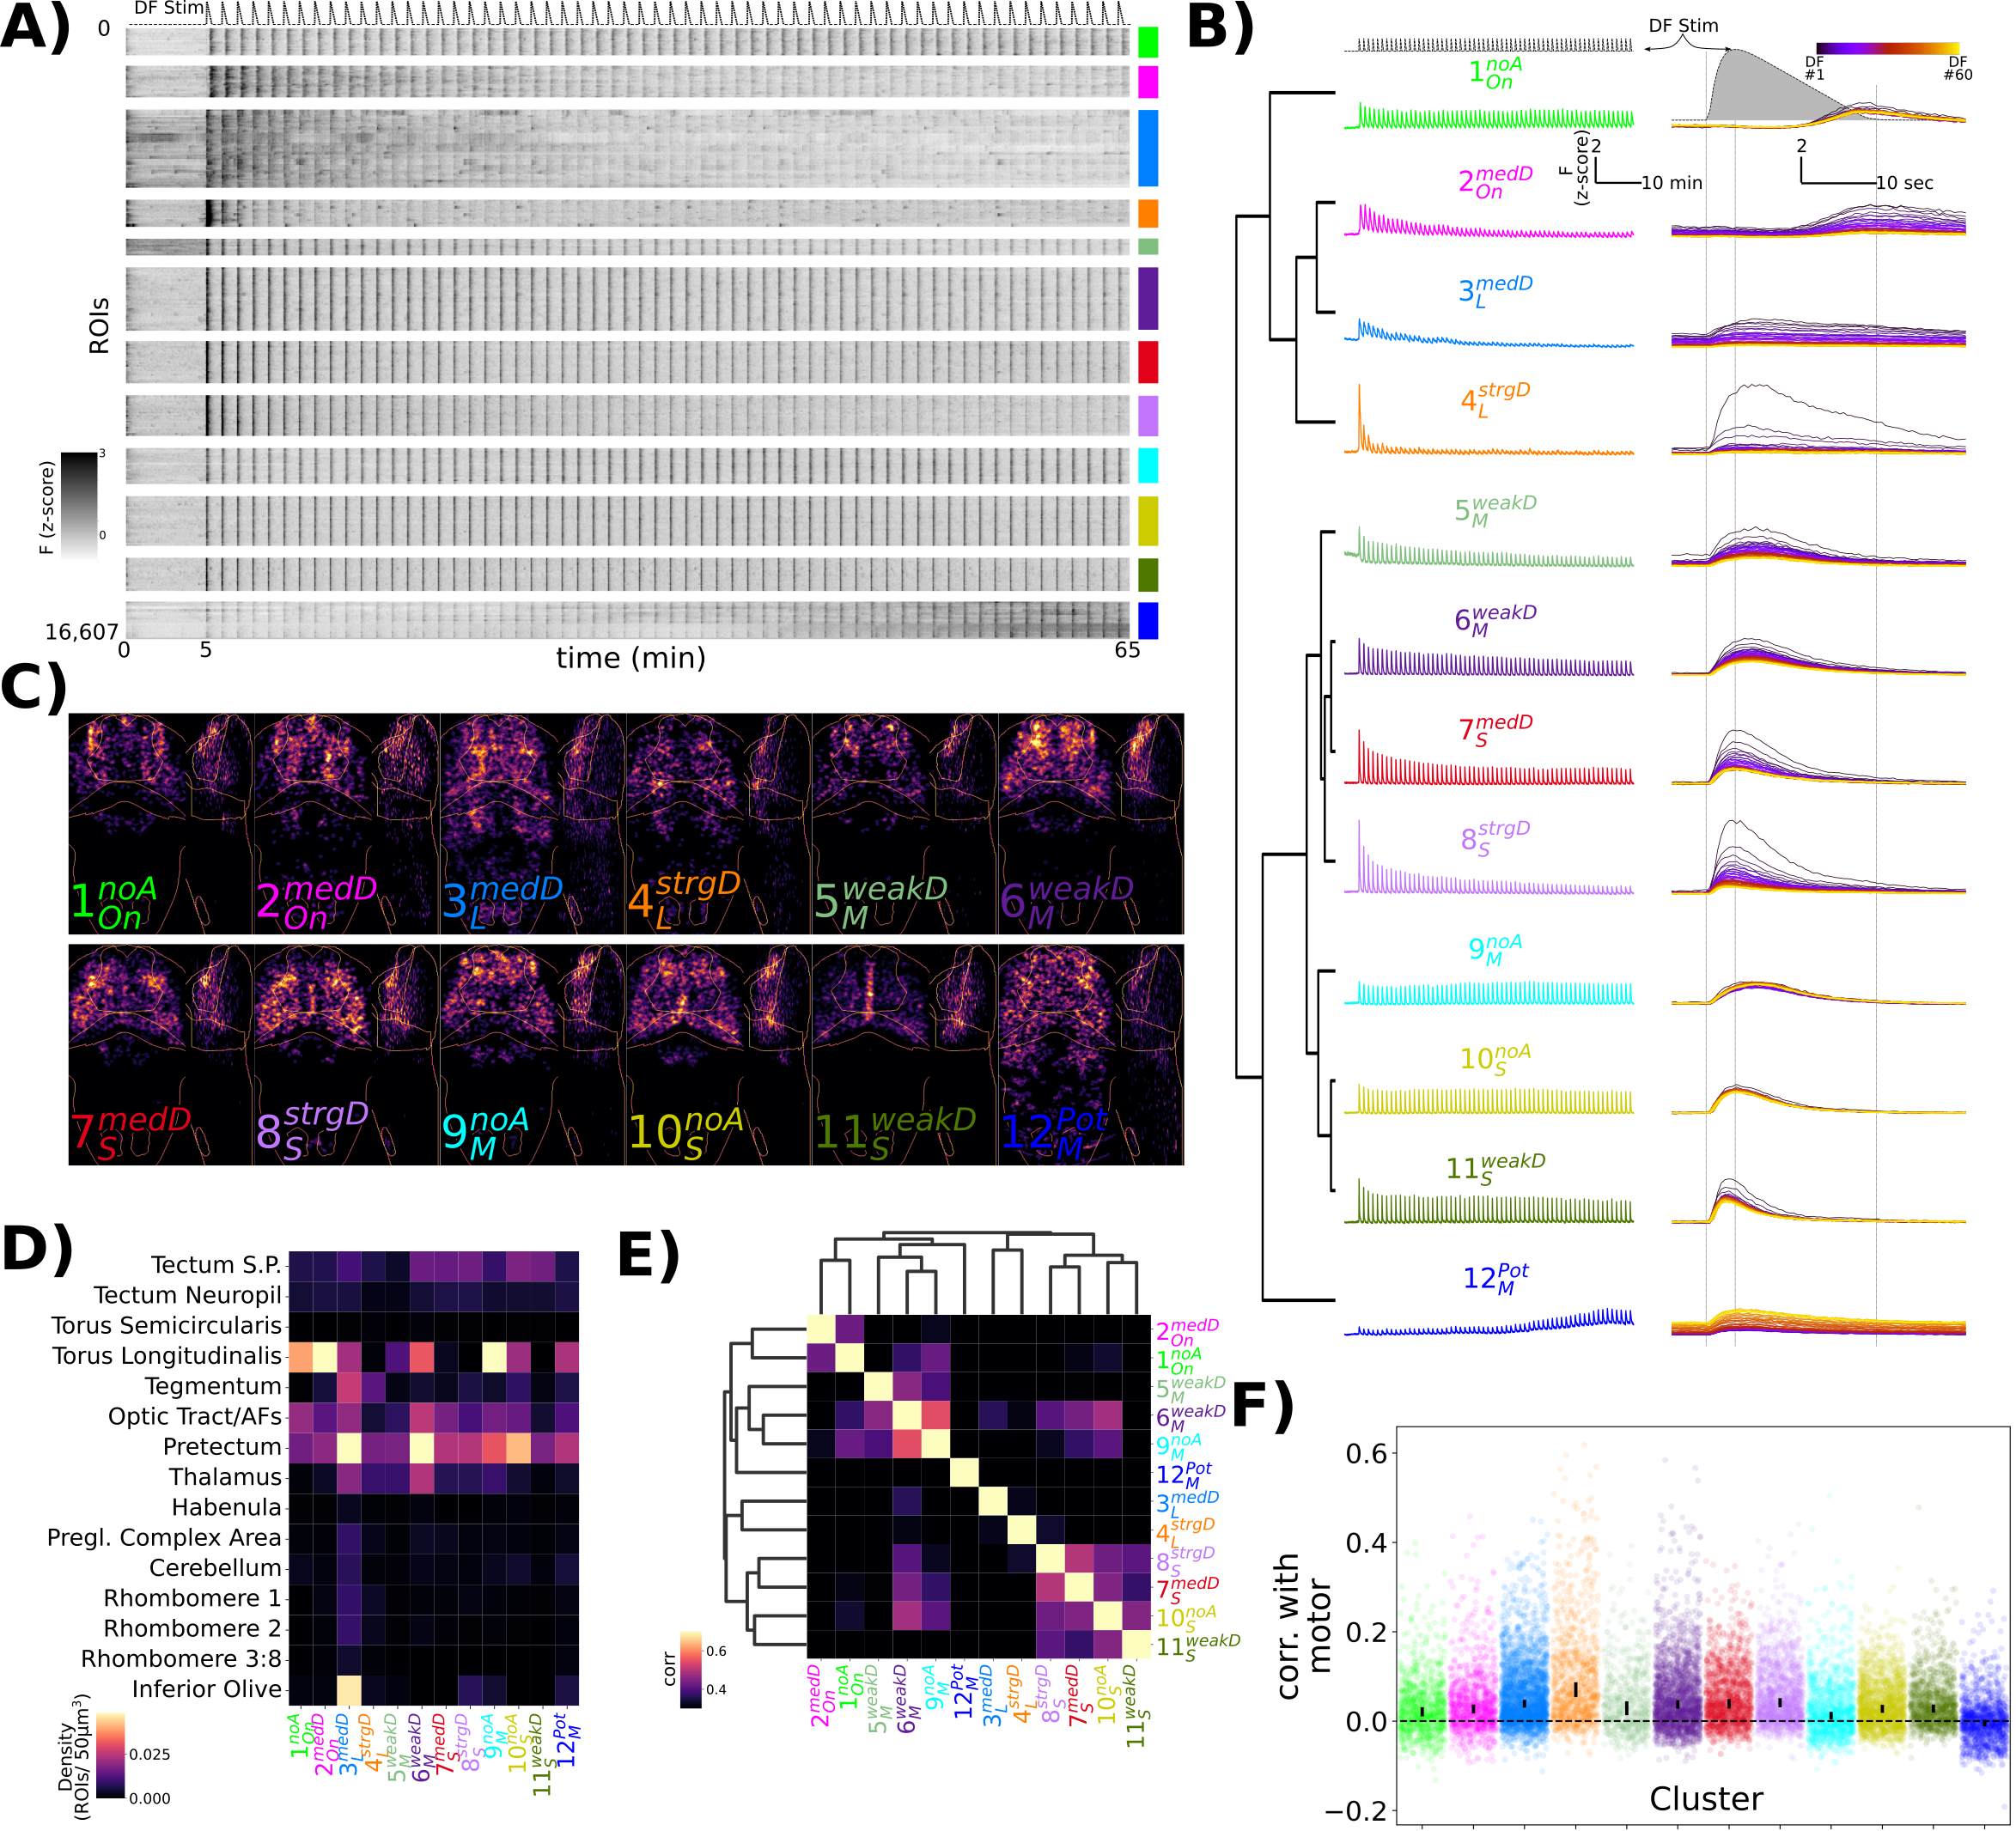
\includegraphics[width=0.95\linewidth]{Figure6 - Clustering.png}
\caption{
Characterization of functional response types during habituation learning 
\textbf{A)} Heatmap of the response profiles of ROIs categorized into 12 functional clusters. n=16,607 ROIs from 34 larvae. 
\textbf{B)} Average z-scored fluorescence each functional cluster plotted for the whole experiment (left column), and centered on each DF stimulus (right column), demonstrating the differences in both adaptation and response shape for each cluster. Clusters were identified using Affinity Propagation clustering (affinity = Pearson correlation, damping = 0.9, preference =-9), and organized using Hierarchical clustering, distance = complete, correlation. Dashed lines in top panels are the DF stimulus convolved with a kernel approximating H2B-GCaMP7f kinetics, used as the regressor in the analysis. 
\textbf{C)} Summed intensity projection of the ROIs belonging to each functional cluster in Z-Brain coordinate space depicting their physical locations in the brain. Projection images are normalized to the maximum value. 
\textbf{D)} Heatmap depicting the density of each cluster that is found within different Z-Brain regions. 
\textbf{E)} Correlogram calculated from the Pearson correlation in downsampled volumes for the ROI centroid positions for each cluster (see Methods). Hierarchical clustering, distance = complete, correlation. 
\textbf{F)} Correlation between motor events and the Ca\textsuperscript{2+} traces for each ROI assigned to the functional clusters. dots = individual ROIs, bar height = 99.99999\% confidence interval around the median value. 
}
\label{fig:6}
\end{center}
\end{fullwidth}
\end{figure}

To categorize the functional heterogeneity within the DF-tuned neurons we used affinity propagation clustering. This method has the advantage that cluster number does not need to be defined beforehand, and attempts to identify the most representative response profiles algorithmically \cite{Forster2020-lg}.  This identified 12 clusters that differed both in their adaptation to repeated DFs, as well as the shape of their response to the DF (\autoref{fig:6}A,B). 

We therefore use these two dimensions of the response to label the clusters:

\subsubsection{Adaptation Profile:  (Depression vs. Potentiation)}


\begin{description}
\item[No Adaptation = $^{noA}$ ]    : 	Cluster 1, 9, 10
\item[Weak Depression = $^{weakD}$ ]    : 	Cluster 5, 6, 11
\item[Medium Depression = $^{medD}$ ]    : 	Cluster 2, 3, 7
\item[Strong Depression = $^{strgD}$ ]    : 	Cluster 4, 8
\item[Potentiation = $^{Pot}$ ]    : 	Cluster 12
\end{description}



\subsubsection{Response Shape: (Transient/Short vs. Sustained/Long)}
\begin{description}
\item[On-response = $_{On}$]    : 	Cluster 1, 2
\item[Long/sustained response = $_{L}$]    : 	Cluster 3, 4
\item[Medium-length response = $_{M}$]    : 	Cluster 5, 6, 9
\item[Short/transient response = $_{S}$]    : 	Cluster 7, 8, 10, 11

\end{description}
\\
\subsubsection{Yielding clusters: $1_{On}^{noA}$, $2_{On}^{medD}$, $3_{L}^{medD}$ , $4_{L}^{strgD}$, $5_{M}^{weakD}$, $6_{M}^{weakD}$, $7_{S}^{medD}$, $8_{S}^{strgD}$, $9_{M}^{noA}$, $10_{S}^{noA}$, $11_{S}^{weakD}$, and $12_{M}^{Pot}$}

\vspace{5mm}
While these results indicate that a dozen functionally distinct neuron types are associated with DF habituation, such cluster-based analyses will force categories upon the data irrespective of if such categories actually exist. To determine if our cluster analyses identified genuine neuron types, we analyzed their anatomical localization (\autoref{fig:6}C, D). Since our clustering was based purely on functional responses, we reasoned that anatomical segregation of these clusters would be consistent with the presence of truly distinct types of neurons. Indeed, we observed considerable heterogeneity both within and across brain regions. For example: 
$11_{S}^{weakD}$was mostly restricted to medial positions within the optic tectum; 
$3_{L}^{medD}$ and $4_{L}^{strgD}$ were more prevalent within motor-related regions of the brain including the Tegmentum and Hindbrain Rhombomeres; 
$9_{M}^{noA}$ was the most prominent cluster in the torus longitudinalis, consistent with the presence of non-habituating signals in the area (\autoref{fig:5}G,H). 

We then quantified the similarity in the spatial relationships among the clusters by looking at the correlations in the positions of the ROIs in downsampled super-voxels of the Z-Brain (\autoref{fig:6}E). This revealed similar hierarchical relationships to those identified functionally (\autoref{fig:6}B), especially with respect to Response Shape, indicating that physical proximity is predictive of the functional similarity of neurons, even across clusters. 

Finally, since our functional analysis was performed purely based on correlations with the DF stimuli, we asked to what extent neurons belonging to each cluster were correlated with motor output. This identified $4_{L}^{strgD}$ as the most strongly correlated to motor output, consistent with its strong habituation profile and its localization within motor-regions of the hindbrain. This indicates that $4_{L}^{strgD}$ neurons likely occupy the most downstream positions within the sensory-motor network. 

These results highlight a diversity of functional neuronal classes observed during DF habituation. Whether there are indeed 12 classes of neurons, or if this is an over- or under-estimate, awaits a full molecular characterization. However, we proceed under the hypothesis that these clusters define neurons that play distinct roles in the DF response and/or its modulation during habituation learning. 
\pagebreak
\subsection{Identification of GABAergic inhibitory neurons during habituation}

\begin{figure}
\begin{fullwidth}
\begin{center}
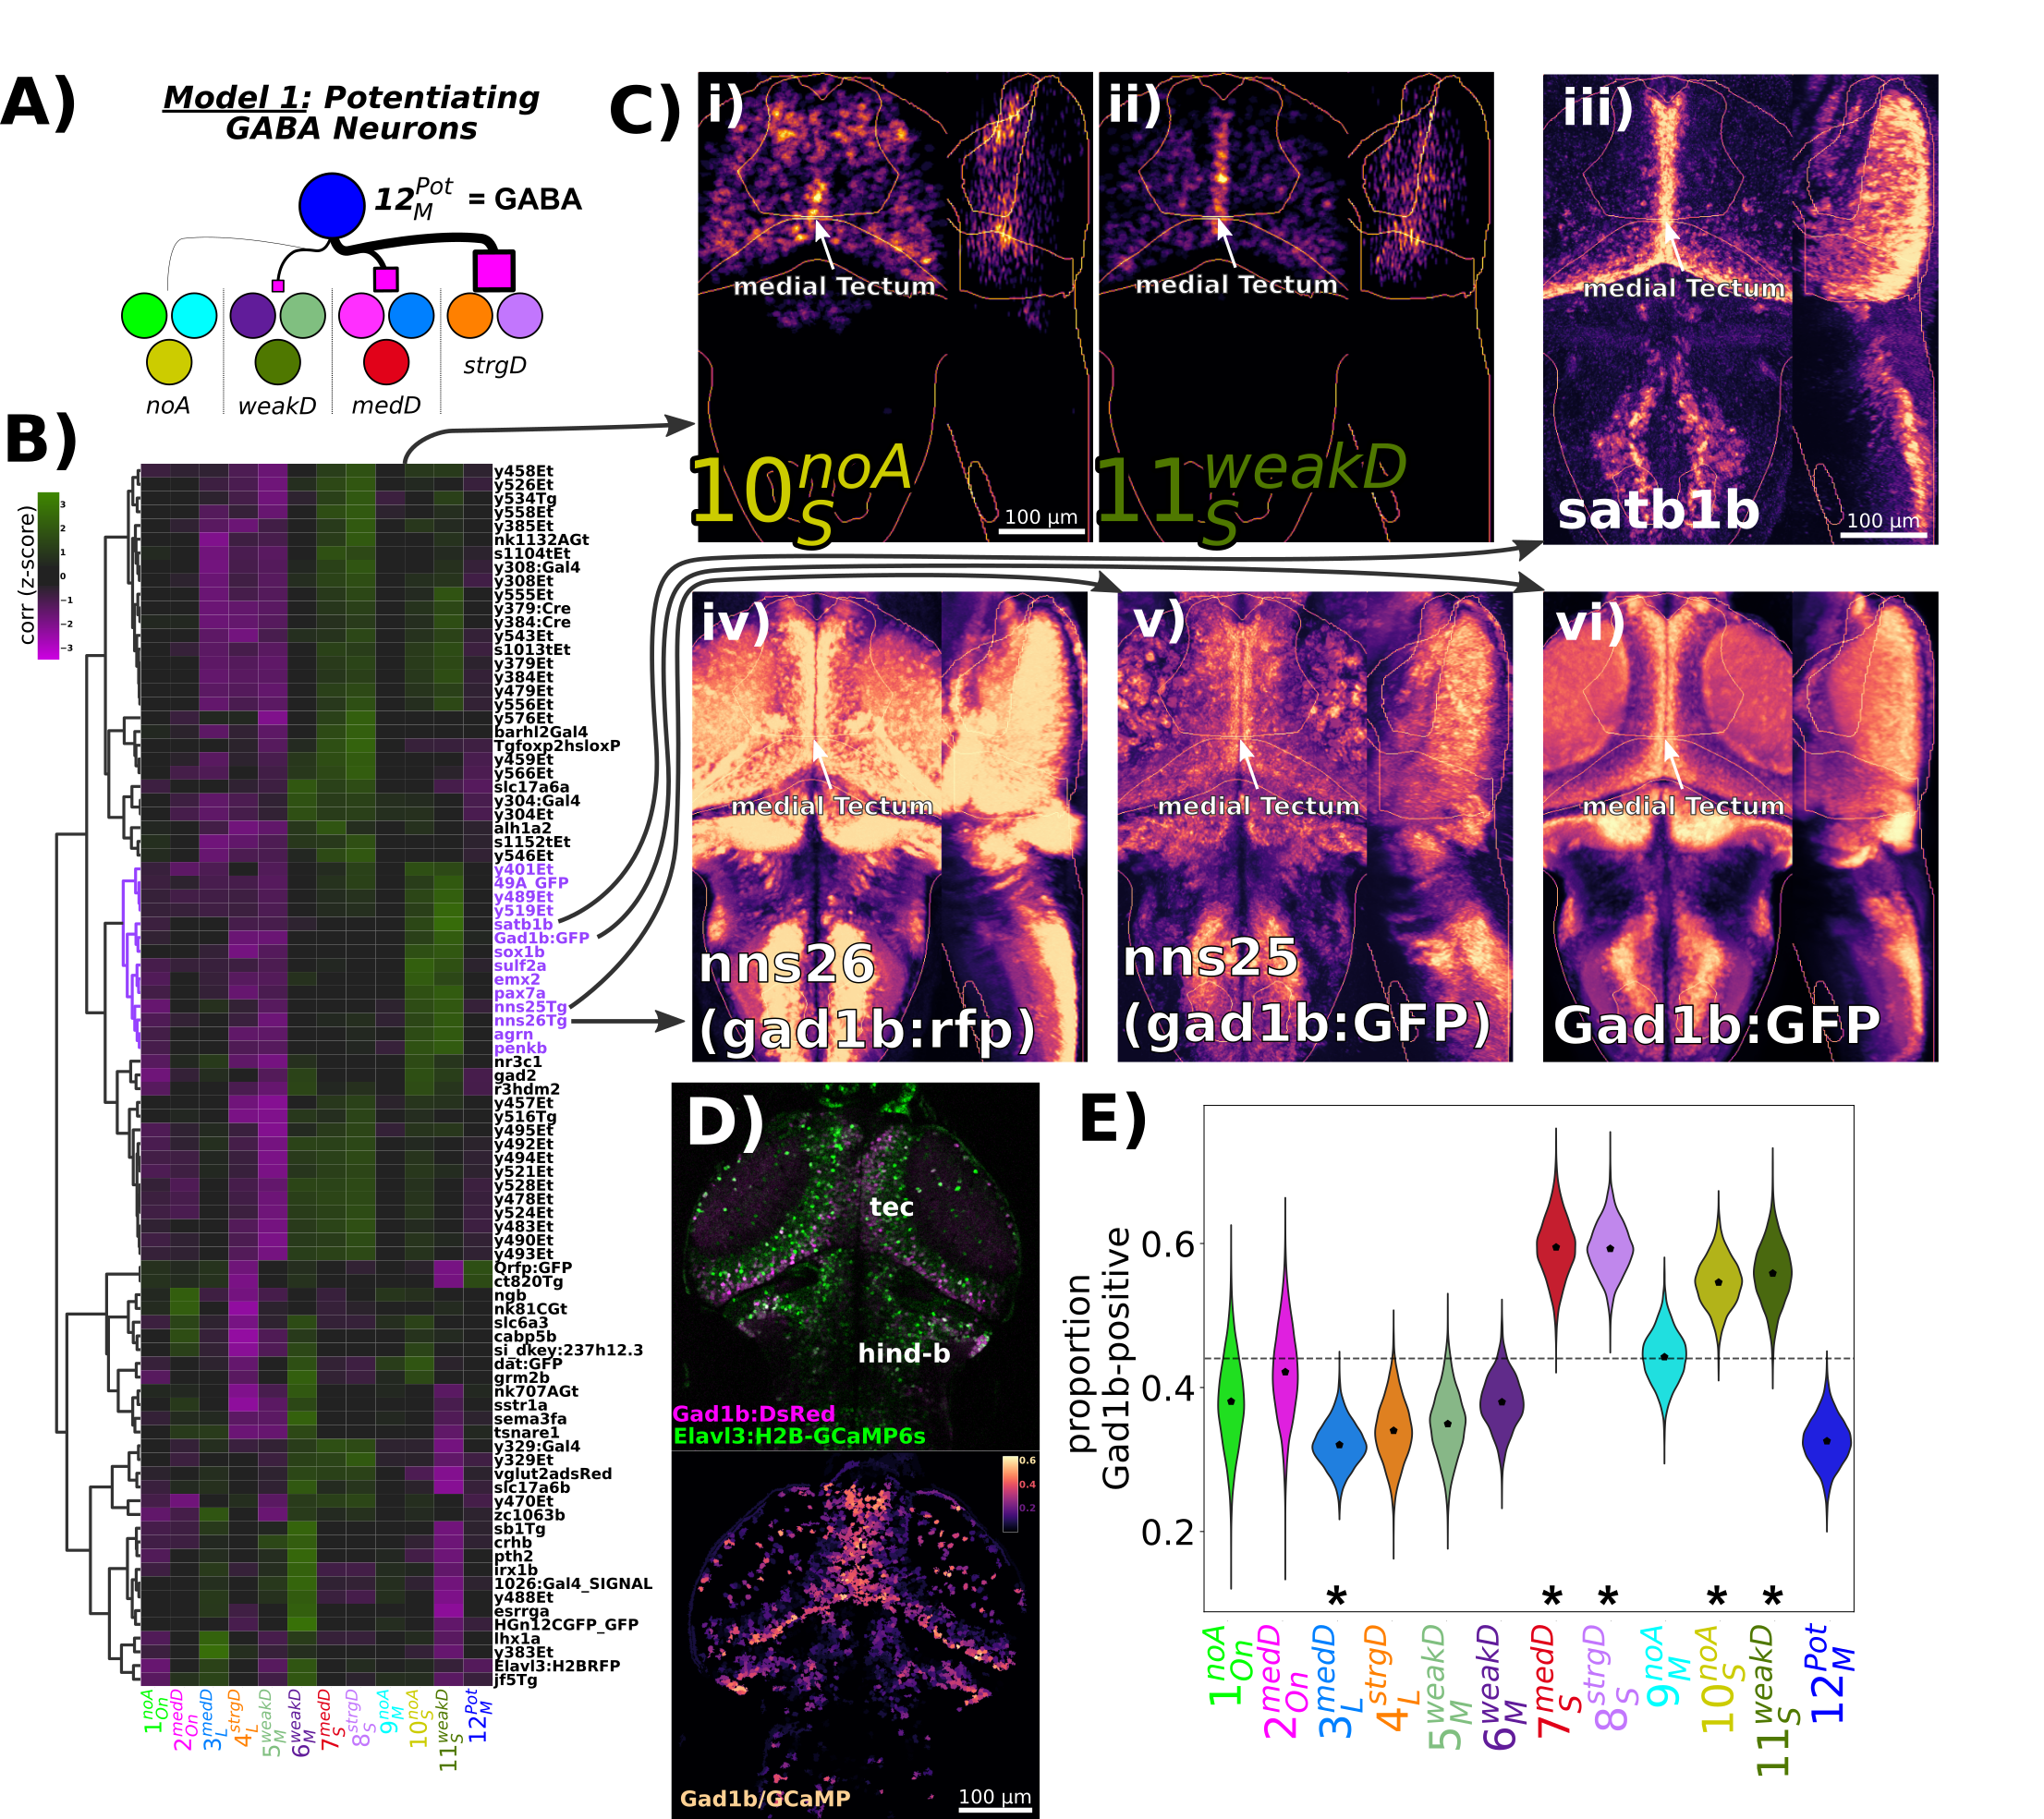
\includegraphics[width=0.99\linewidth]{Figure7-GABA.png}
\caption{
An atlas-based search for molecular markers identifies GABAergic neuronal classes. 
\textbf{A)} \underline{Model 1}, proposed to explain how potentiating GABAergic inhibition could mediate the range of depressive adaptations observed during habituation. Model posits that the sensitizing neurons are GABAergic ($12_{M}^{Pot}$, blue), and they differentially connect to functional subtypes: Strong connectivity to strongly habituating classes, weak connectivity to weakly habituating classes, etc. 
\textbf{B)} Hierarchically clustered heatmap depicting the correlation of markers aligned to the Z-Brain atlas with the spatial arrangement of the 12 functional clusters  (distance = complete, correlation). Correlation values are z-scored by rows to highlight the cluster(s) most strongly correlated or anti-correlated with a given marker. The subset of the hierarchy containing the gad1b-reporters is coloured in purple. 
\textbf{C)} Normalized summed intensity projections comparing the spatial arrangements of i) $10_{S}^{noA}$, and ii) $11_{S}^{weakD}$
with atlas markers found within the the purple cluster
iii) satb1b HCR (Shainer et al., 2022), MapZeBrain Atlas
iv) nns25, aka TgBAC(gad1b:GFP) (Satou et al., 2013), MapZeBrain Atlas
v) nns26, aka TgBAC(gad1b:LOXP-RFP-LOXP-GFP) (Satou et al., 2013), MapZeBrain Atlas
vi) TgBAC(gad1b:GFP) (Satou et al., 2013), Z-Brain Atlas
\textbf{D)} 2-photon imaging of Tg(Gad1b:DsRed);Tg(elavl3:H2B-GCaMP6s) larvae depicting the raw data for each channel (top), and the ratio of Gad1b/GCaMP6s fluorescence in each ROI functionally identified using suite2p. 
\textbf{E)} ROIs imaged in double transgenic larvae are assigned a cluster identity based on their correlation to the cluster mean trace, and classified as Gad1b-positive based on a Gad1b/GCaMP6s ratio of greater than 0.25. Dotted line = expected proportion based on total number of cells classified as Gad1b-positive. *=p<0.05, Chi Square test with Bonferroni correction. Distributions underlying violin plots calculated by bootstrapping 5000 replicates. n = 1835 ROIs in 6 larvae. 
}
\label{fig:7}
\end{center}
\end{fullwidth}
\end{figure}

How might the functional classes of neurons we identified interact within a circuit to drive habituation behaviour? Considering that we have implicated GABAergic inhibition in habituation, the simplest model would assign a GABAergic identity to the potentiating neurons; $12_{M}^{Pot}$. These inhibitory neurons would then act to progressively increase inhibition during learning (\autoref{fig:7}A, \underline{Model 1}). Potentiation of these neurons could be achieved through, for example, LTP at their inputs during learning. 

A limitation of the pan-neuronally expressed GCaMP imaging approach is the lack of knowledge as to the molecular identity of neurons, such as neurotransmitter type. Virtual co-localization analyses with 3D atlases can be used to identify candidate molecular markers for functionally identified neurons, provided sufficient stereotypy exists in neuronal positioning, and the relevant marker exists in the atlas \cite{Dunn2016-vt, Randlett2015-hy}. Therefore, we analyzed the spatial correlations for markers contained in the Z-Brain \cite{Randlett2015-hy}, zebrafish brain browser \cite{Gupta2018-ik, Marquart2017-na, Tabor2018-bw}, and MapZeBrain atlases \cite{Kunst2018-az, Shainer2022-sn}. We identified markers showing the highest spatial correlations with any of our functional clusters (corr. > 0.15, n=89 of 752 markers), and organized these hierarchically (\autoref{fig:7}B).

We were particularly interested in associations with GABAergic neurons labeled by the gad1b reporter lines. These were located in a region of the hierarchy showing greatest spatial similarity with $10_{S}^{noA}$ and $11_{S}^{weakD}$(\autoref{fig:7}C). An enrichment along the medial Tectum is common to markers in this region of the hierarchy, where the highest density of GABAergic neurons within the Tectum reside. Contrary to \underline{Model 1}, $12_{M}^{Pot}$ neurons did not appear to be associated with GABAergic neuronal markers in this analysis.  

These data indicated that $10_{S}^{noA}$ and $11_{S}^{weakD}$neurons are the predominant GABAergic classes. To test this, we imaged the response of neurons in Tg(Gad1b:DsRed);Tg(elavl3:H2B-GCaMP6s) double transgenic larvae,  and classified neurons as gad1b-positive or -negative based on DsRed/GCaMP levels (\autoref{fig:7}D). Indeed we saw a heterogeneous distribution of Gad1b-positive neurons across functional clusters, including a significant enrichment in not only $10_{S}^{noA}$ and 11SweakD, but also the other two clusters with the “Short” Response Shape ($7_{S}^{medD}$ and $8_{S}^{strgD}$, \autoref{fig:7}E). The remaining clusters either showed no significant bias, indicating that they contain mixed populations, or a significant depletion of gad1b-positive cells, suggesting that they comprise mostly of excitatory or neuromodulatory neurons ($3_{L}^{medD}$ and $12_{M}^{Pot}$). 

Therefore, these results are inconsistent with Model 1, since $12_{M}^{Pot}$ neurons appear to be mainly non-GABAergic. Instead, GABAergic neurons span the remainder of the range of adaptation profiles, from non-adapting to strong-depression. These neurons are best characterized by the shape of their response to the stimulus, perhaps reflecting a transient bursting style of activity relative to other neuronal types that exhibit more sustained firing patterns. 

\subsection{A pharmacologically-constrained model of the habituating circuit}

\begin{figure}
\begin{fullwidth}
\begin{center}
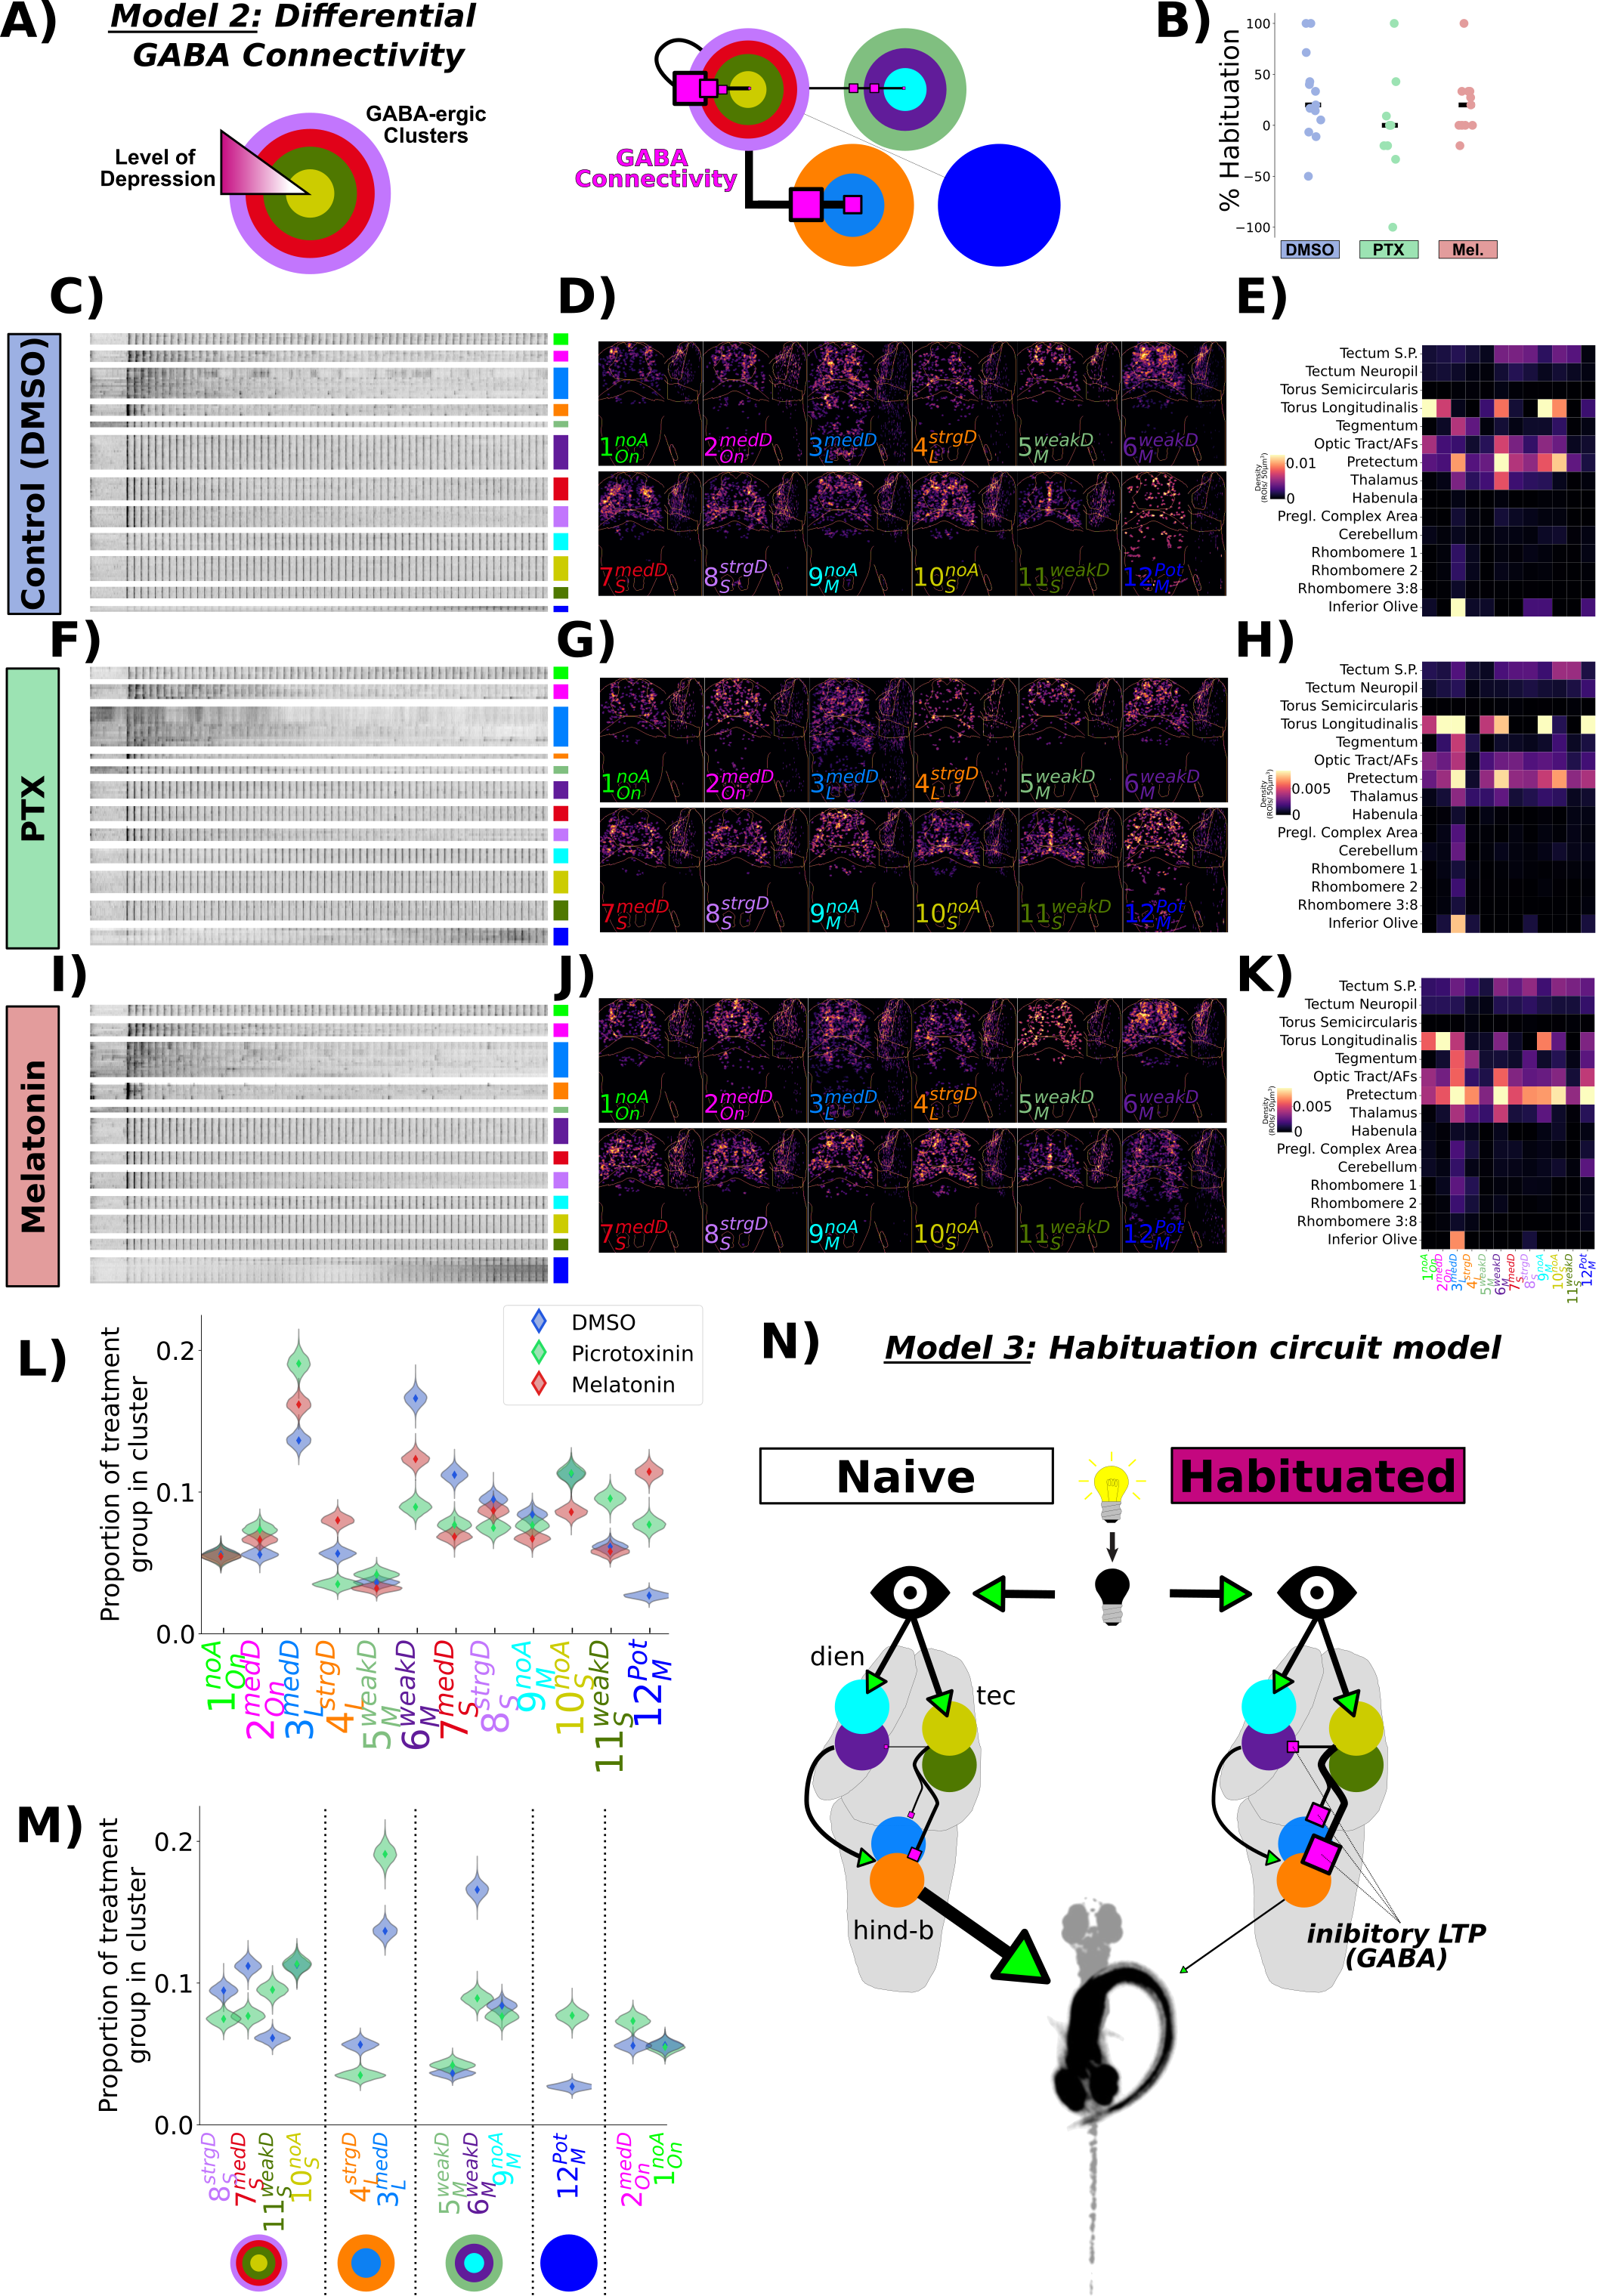
\includegraphics[width=0.6\linewidth]{Figure8 - Drugs.png}
\caption{
A pharmacologically constrained model for dark flash habituation
\textbf{A)} \underline{Model 2}, proposed to explain how biased GABAergic inhibition could mediate the differential habituation rates observed across functional classes of neurons. Model proposes that the neurons with the Sort Response shape are GABAergic, and that they differentially connect to the other functional subtypes, as well as themselves to drive the response decreases observed during habituation. The strength of this inhibitory connectivity determines the decrease in responsiveness across neuronal classes. Larger pink box = Stronger inhibition. 
\textbf{B)} Percent habituation for larvae during Ca\textsuperscript{2+} imaging, calculated as:
$Percent Habituation = 
100 * (1 - \frac{P(Resp_{31\rightarrow60})}{0.5*(P(Resp_{1\rightarrow30} + P(Resp_{31\rightarrow60}))})$
\textbf{C-K)} Functional clustering of neurons from larvae treated with DMSO (vehicle control), Picrotoxinin (PTX, 10uM), or Melatonin (1uM). 
C,F,I) Heatmap of response profiles of ROIs categorized into the 12 functional clusters. 
D,G,J) Summed intensity projection of the ROIs belonging to each functional cluster in Z-Brain coordinate space depicting their physical locations in the brain. Projection images are normalized to the maximum value. 
E,H,K) Heatmap depicting the density of each cluster that is found within different Z-Brain regions.
C-E) DMSO, n = 428,720 total ROIs in 14 larvae F-H) Picrotoxinin (PTX), n = 271,037 total ROIs in 9 larvae I-K) Melatonin treatment, n = 350,516 total ROIs in 11 larvae.
\textbf{L)} Proportion of neurons belonging to each functional cluster across treatment groups. Distributions for violin plots are bootstrapped from 5000 replicates. 
\textbf{M)} Same data as M, only showing the data for PTX vs DMSO vehicle control, re-ordered to reflect the cluster Adaptation Profiles. 
\textbf{N)} \underline{Model 3}, proposed circuit model for the habituation of the probability of responding to a DF stimulus. The dark flash stimulus is detected by the retina and sent as an unadapted signal to the brain. GABA-ergic inhibitory neurons form the critical node in the habituating circuit, where habituation occurs as the result of a potentiation of GABAergic synapses, resulting in depressed responses in connected neurons. The strength of neuronal adaptation during habituation depends on the GABAergic connectivity strength (as in  \underline{Model 2} (A)). The output neurons of the circuit are the Long-responding class. Potentiated GABAergic inhibition onto this population silences behavioural output. 
}
\label{fig:8}
\figsupp[Mean response of functionally identified clusters after different pharmacological treatments]
{Mean response of functionally identified clusters after different pharmacological treatments.
\textbf{A-C)} Average z-scored fluorescence each functional cluster plotted for the whole experiment (left column), and centered on each DF stimulus (right column), demonstrating the differences in both adaptation and response shape for each cluster after treatment with \textbf{(A)} 0.1\% DMSO vehicle control, \textbf{(B)} Picrotoxinin (10uM), or \textbf{(C)} Melatonin (1uM). 
\textbf{D)} Same data as A-C, plotted together for each treatment group.
}{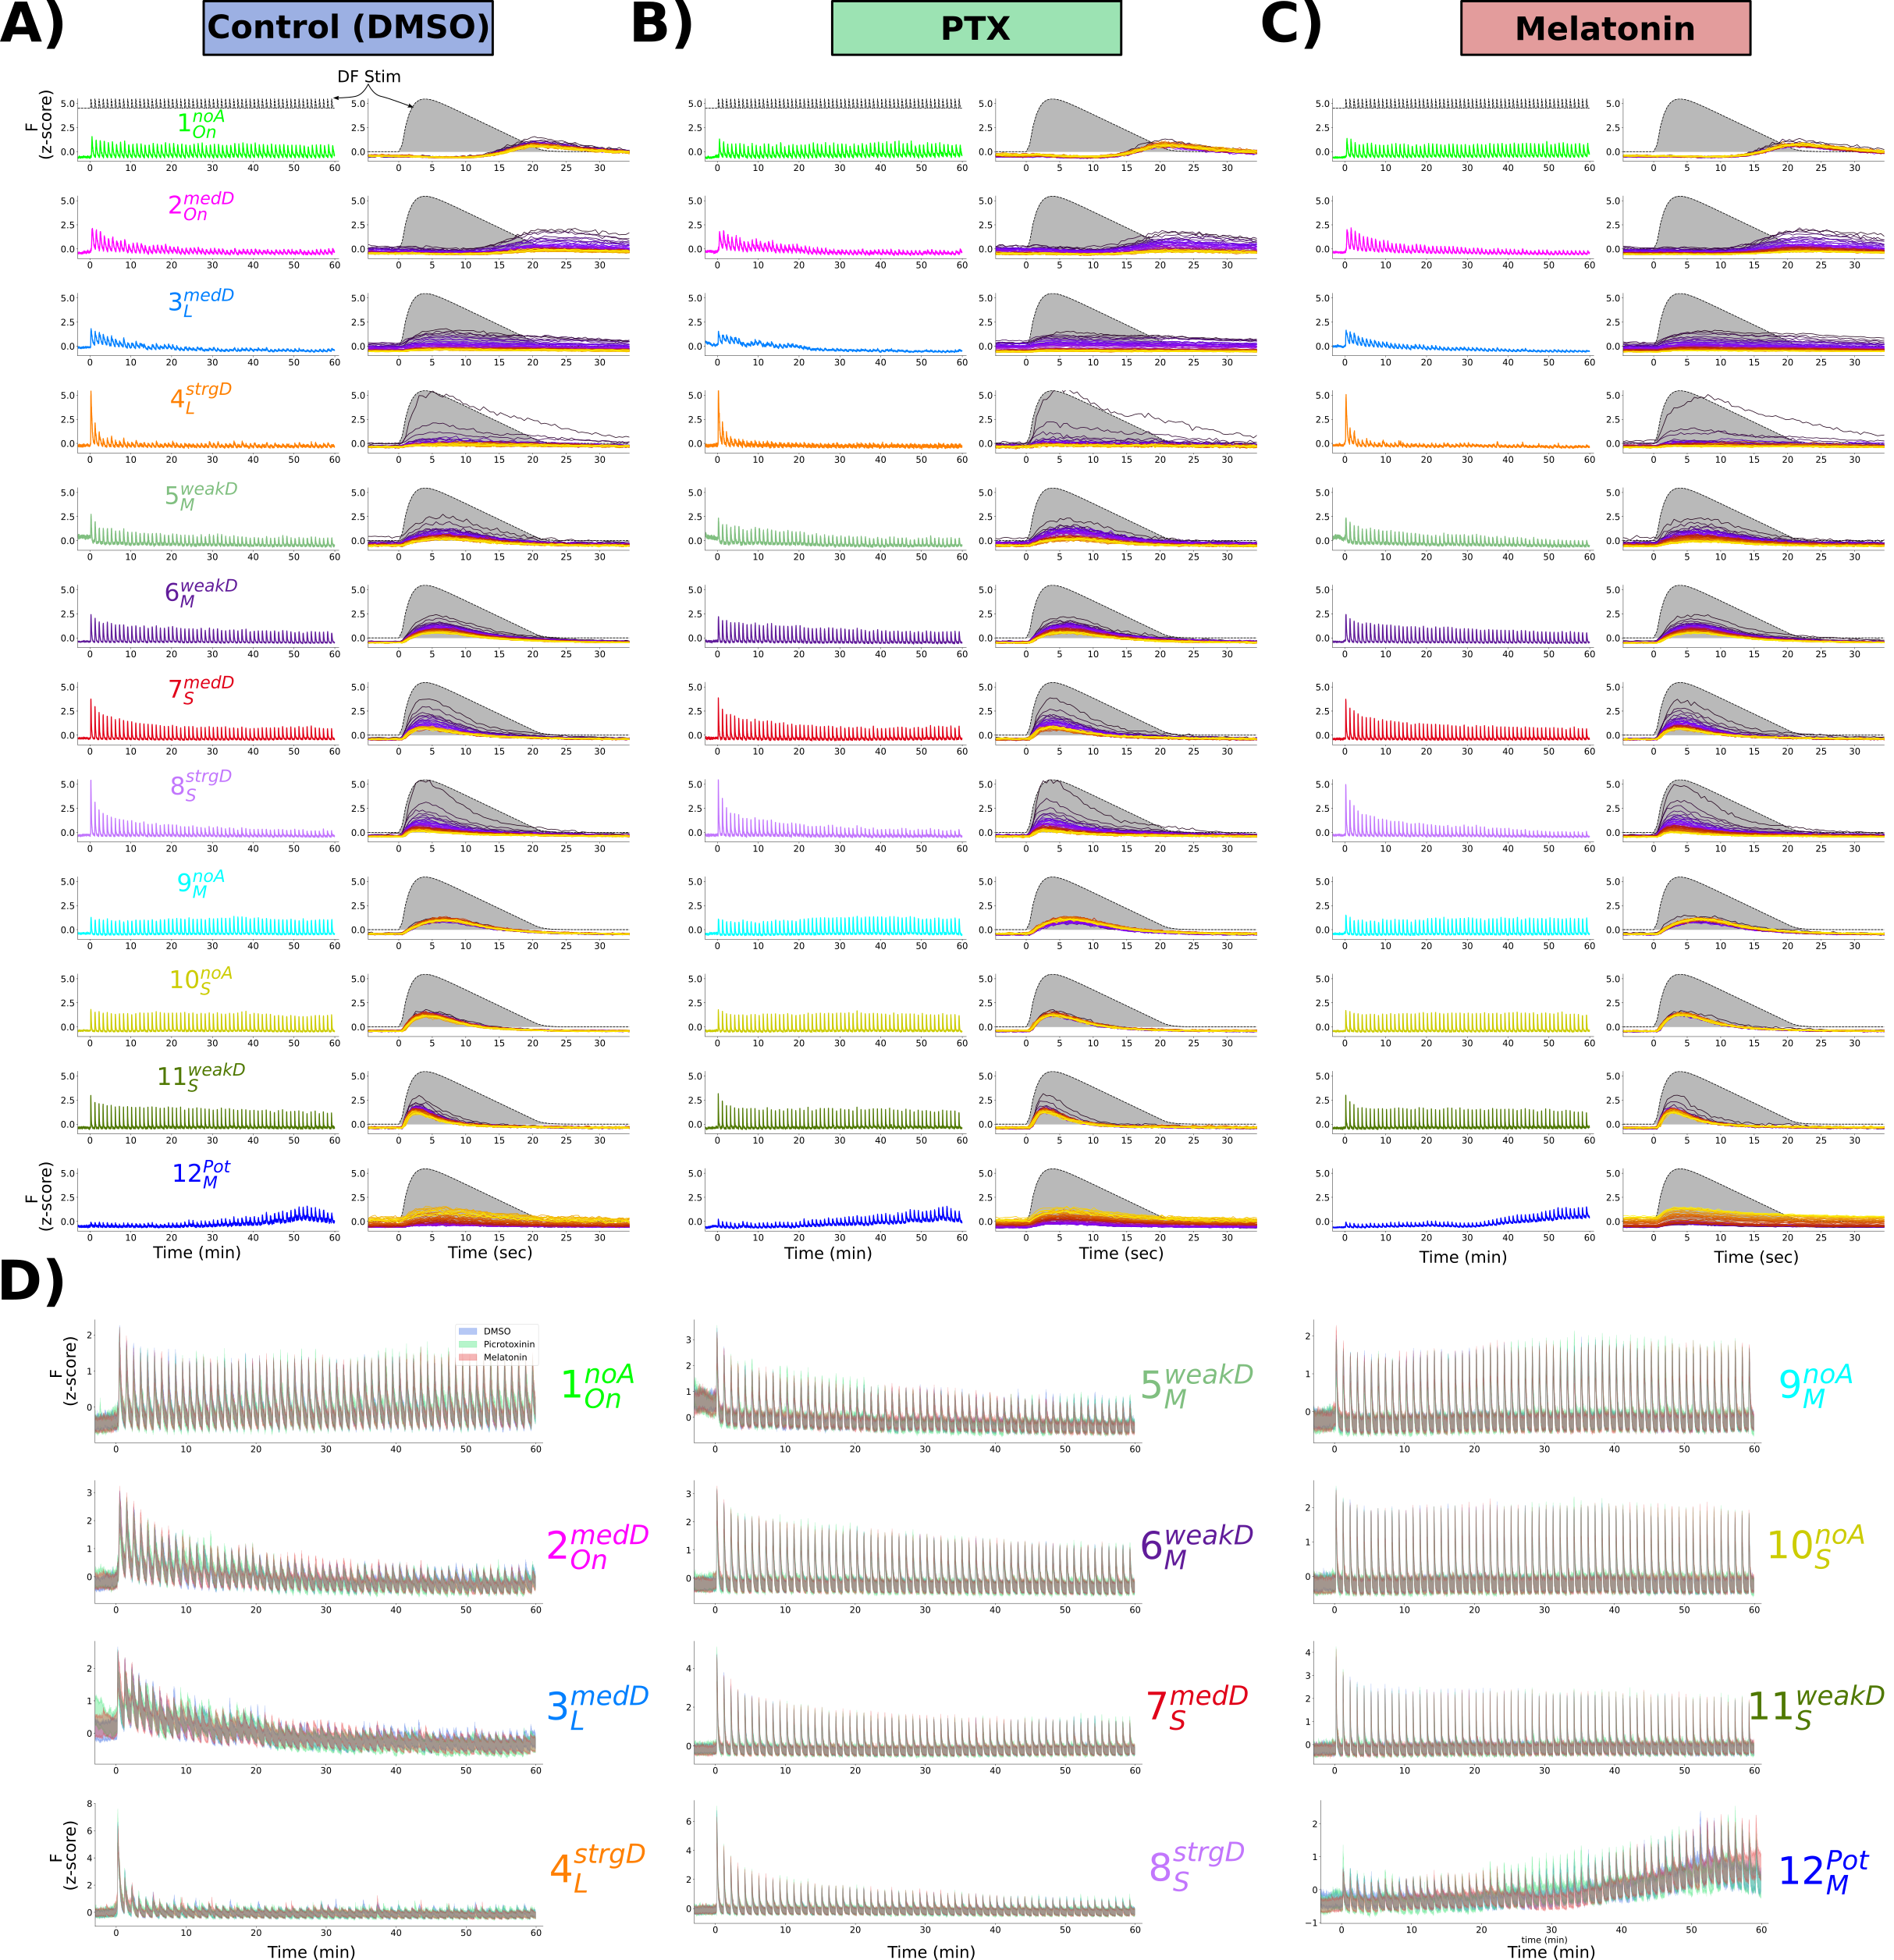
\includegraphics[width=14cm]{FigureS3_DrugsMeanVectors.png}}
\label{fig:S8}
\end{center}
\end{fullwidth}
\end{figure}


Our functional and anatomical analyses indicate that distinct populations of GABAergic neurons exist that inhibit behavioural responsiveness during learning. What connectivity and plasticity mechanisms might underlie the relationships between these neurons, and how do they shape the functional patterns of other neurons in the circuit? We currently do not have sufficient anatomical knowledge to realistically constrain such models. However, if we approach this problem with Occam's razor with respect to the mechanism of plasticity we arrive at a model in which the global potentiation of GABAergic synapses drives habituation. Potentiation of GABA-ergic output through inhibitory long-term potentiation (i-LTP) could explain why GABAergic neurons do not potentiate in their firing pattern, but still exhibit increasing influence over the circuit during habituation. Assuming that excitatory activation in the circuit is consistent, differential connectivity weights between GABAergic neurons and the other neuronal classes could drive the differential rates of depression: i-LTP at strong GABAergic connections drives strong depression, while i-LTP at weak GABAergic connections drives weak depression (\autoref{fig:8}A, \underline{Model 2}). 

To test this model, we asked how PTX and Melatonin influence the dynamic activity states in different classes of neurons. Antagnoism of GABA receptors via PTX should decrease the influence of these inhibitory neurons on the remaining populations, shifting the balance from strong depression towards weaker or non-adapting response profiles. We have found that Melatonin potently increases habituation behaviour (\autoref{fig:3}), and further depresses brain-wide neuronal activity during habituation beyond normal levels (\autoref{fig:4}). These are effectively opposite of the effect of PTX, and thus we hypothesized that Melatonin acts in opposition to GABA in the circuit, shifting the balance towards strongly habituating profiles. This model of the action of Melatonin also fits with the observations that Melatonin can directly potentiate the effects of GABA \cite{Cheng2012-gv, Niles1987-oc}. Alternatively Melatonin may signal through one of 6 known G-protein coupled receptors in larval zebrafish \cite{Maugars2020-pz}, which could act to modulate activity states in GABAergic neurons or their targets. 

We compared the Ca\textsuperscript{2+} activity patterns in neurons from fish treated with vehicle (0.1\% DMSO), PTX, or Melatonin (\autoref{fig:8}B-M). At the behavioural level, we found a trend indicating that we were able manipulate habituation pharmacologically in our tethered imaging assay, though this was not statistically significant (\autoref{fig:8}B). This discrepancy relative to the very strong behavioural effects in freely-swimming animals (\autoref{fig:3}) likely result from the head-restrained protocol, which itself strongly inhibits behavioural output. Therefore assaying for habituation at the behavioural level is difficult to interpret. Alternatively, drug access to the brain may have been compromised by the agarose mounting resulting in weaker behavioural effects. Yet, since we did observe a trend in behavioural data, we proceeded under the assumption that the drugs were having the desired effects. 

We examined the activity profiles of neurons that belonged to the 12 different functional clusters. Surprisingly, we observed no strong alterations of the response profiles of these neurons (\autoref{fig:8}C-K, \autoref{fig:8}-\autoref{fig:S8}). However, what was clearly altered was the proportion of neurons that belonged to different functional classes (\autoref{fig:8}L,M).

From these analyses we conclude the following:

\begin{description}
\item[A)]
The pharmacological manipulations did not alter the activity of neurons in such a way as to alter the average activity states of the population within each cluster (\autoref{fig:8}-\autoref{fig:S8}). Instead, the proportion of neurons belonging to different functional classes changed. This may result from our classification scheme, or could point to fixed and relatively inflexible processing strategies that the brain is using in the context of dark-flash habituation.
\item[B)]
The effect of PTX on cluster reassignment generally followed the type of effects predicted from Model 2, increasing the proportion of cells falling into the weaker depressing classes (\autoref{fig:8}M). This pattern was most clear in the classes with “Short” and “Long” response shapes, which are those that included the Strongly depressed classes of neurons, and would thus be the most influenced by GABA-mediated inhibition. Non-depressing classes were not strongly modulated, consistent with a model that these neurons receive little GABAergic input. Therefore, we conclude that Model 2 is consistent with much, but not all of the alternations in response to PTX. For example, PTX increased the proportion of $6_{M}^{weakD}$ neurons, which does not follow from \underline{Model 2}.
\item[C)] 
Based on our hypothesis that the effect of Melatonin is to potentiate GABA-ergic inhibition, we expected PTX and Melatonin to have opposite effects. Similar to (B), this hypothesis is not fully supportedby all of the data, but is consistent with the observations in a subset of functional classes, perhaps those that are most critical for the habituation of response probability. Indeed, the expected opposite effects of PTX and Melatonin were present in two of the most conspicuous functional classes: $4_{L}^{strgD}$, which is most strongly correlated with motor output and thus is most closely associated with behavioural initiation (\autoref{fig:6}F), and 11SweakD, which showed the clearest GABA-like anatomical pattern in the tectum. 
\item[D]
One of the most interesting classes of neurons we observed during habituation are those that potentiate their responses ($12_{M}^{Pot}$). Remarkably, both Melatonin and PTX increased the proportion of neurons within this class. This result, combined with our observation that these cells are non-GABAergic (\autoref{fig:7}E), strongly suggests that the role of these cells is not simply to suppress activity in the circuit to inhibit behavioural responses (as in Model 1). The functional role played by this class of neurons during habituation remains mysterious. However, it may relate to some of the common behavioural effects of Melatonin and PTX, such as the inhibition of habituation when measuring response Displacement (\autoref{fig:3}A,B, \autoref{fig:3}-\autoref{fig:S3}1A) 1E, F). 

\end{description}


Based on these data we propose a working model of the dark flash habituation circuit, particularly focused on the elements we have implicated in the decreasing probability of response (\autoref{fig:8}N, \underline{Model 3}). At the center are the GABAergic synapses, whose progressive potentiation drives habituation. Their influence on the depression of excitatory neurons in the circuit is biased based on their connectivity weights, where strong connectivity drives strong-habituation. Strong silencing of the long-responding motor-related neurons ($4_{L}^{strgD}$) suppresses O-bend responses. PTX acts upon the outputs of the GABAergic neurons to decrease their influence in the circuit, thus inhibiting habituation. Melatonin acts in a similar manner but opposite way, either by directly potentiating the action of GABA at the synapse (Cheng et al., 2012; Niles et al., 1987), or by decreasing the excitability of postsynaptic neurons. 

\section{Discussion}
\subsection{Molecular mechanisms of DF habituation}

In the pharmaco-behavioural data resulting from our screen, we focused our analysis on those pharmacological agents and pathways that strongly and relatively specifically modulated habituation when measuring response probability. We found that inhibition of GABAA/C Receptors using PTX reduced habituation learning. GABA is the main inhibitory neurotransmitter in the zebrafish brain, and deficits in GABA signaling lead to epileptic phenotypes \cite{Baraban2005-xq}. We were fortunate that our screening concentration (10\muM) did not induce seizures, but was still sufficient to inhibit habituation. This implies that the habituation circuit is exquisitely sensitive to changes in GABA signaling at levels well below the threshold required to globally change excitatory-inhibitory balances. This argues for a central rather than supporting role of GABAergic inhibition in dark-flash habituation. 

A critical role for GABA in habituation is consistent with data from \emph{Drosophila}, where both olfactory and gustatory habituation have been linked to GABAergic interneurons \cite{Das2011-gd, Paranjpe2012-ce,Trisal2022-pa}. Therefore, this circuit motif of increasing inhibition to drive habituation may be a conserved feature of habituation, which would allow for a straightforward mechanism for habituation override during dis-habituation via dis-inhibition \cite{Cooke2020-mz, Trisal2022-pa}. 

Our screen also identified that neuro-hormonal signaling is critical for habituation, where Melatonin and Estrogen receptor agonists potently increase habituation learning rate. The role of Estrogens on learning and memory is well established \cite{Luine1998-iz,Nilsson2002-fi}. Though its role in habituation is less well explored, it has previously been shown to increase memory retention for olfactory habituation in mice \cite{Dillon2013-ez}. To our knowledge, Melatonin has not previously been implicated in habituation, though it has been implicated in other learning paradigms \cite{El-Sherif2003-tv, Jilg2019-lq}. Notably, Melatonin was shown to block operant learning at night in adult zebrafish \cite{Rawashdeh2007-ts}, and therefore Melatonin appears to be able to both promote or inhibit plasticity in zebrafish, depending on the paradigm. 

While Melatonin and Estrogen were not strong candidates for involvement in DF habituation plasticity before our screen, their previous associations with learning and memory reinforce the idea that these molecules play critical roles in plasticity processes. In support of this idea, we have previously shown that habituation is regulated in a circadian-dependent manner \cite{Randlett2019-fi}, and both Melatonin and Estrogen levels fluctuate across the circadian cycle \cite{Alvord2022-ii, Gandhi2015-vw, Zhdanova2001-dq}, suggesting that either or both of these pathways may act to couple the circadian rhythm with learning performance. 

Finally, approximately 2\% of the US population use Melatonin as a sleep-aid \cite{Li2022-lu}, and a substantial proportion of US women take Estrogen as part of either oral contraceptives or hormone replacement therapy. Therefore, understanding the roles these molecules play in neuroplasticity is a clear public health concern. 

\subsection{Circuit mechanism of DF habituation}

Using pERK-based whole brain activity profiling, we first identified that habituation learning is associated with a broad depression of neuronal activity. These data appear consistent with a model for habituation in which plasticity early within the visual pathway acts as an activity bottleneck, perhaps even in the retina. However, our Ca\textsuperscript{2+} imaging experiments identified a diverse range of neuronal adaptation profiles, including non-depressing and potentiating neurons spread throughout sensory- and motor- related areas of the brain, inconsistent with such a model. Thus, non-habituated signals are transmitted throughout the brain, indicating the presence of parallel processing streams during habituation. 

This is more consistent with our previous behavioural analyses of habitation, where we postulated that multiple plasticity loci co- exist, arranged in both parallel and series within the circuit \cite{Randlett2019-fi}. Such a model is further supported with brain-wide imaging data for short-term habituation to looming stimuli, where distributed neurons were identified that showed differential rates of habituation \cite{Marquez-Legorreta2022-ih}. It is important to point out that Marquez-Legorreta et al. did not observe non-adapting or potentiating neurons in their experiments. This may be due to differences in analysis methods, or could highlight a difference between short- and long-term habituation circuit mechanisms, the latter of which may rely on more complex circuit mechanisms involving both potentiation and suppression of responses. 

While we do not have enough anatomical data to constrain circuit connectivity models that drive DF habituation, here we demonstrate the  use of pharmacology, functional imaging and neurotransmitter classifications to constrain our models. Specifically, pharmacology indicated a central role for GABA in habituation, and our functional imaging highlighted a role for distinct classes of neuronal types in the DF circuit, including potentiating neurons ($12_{M}^{Pot}$). Initially, this led us to propose a very simple model for habituation, where potentiating neurons are GABAergic and thus progressively inhibit the circuit during learning (\underline{Model 1}). However, in silico co-localization analyses and double transgenic Ca\textsuperscript{2+} imaging identified $12_{M}^{Pot}$ neurons to be  predominantly non-GABAergic, thereby refuting this simple model. Instead, we propose that the GABAergic neurons in the circuit are characterized by their short burst of activity to the stimulus onset, and that the potentiation of their synapses drives habituation (\underline{Model 3}, \autoref{fig:8}N). This a somewhat unexpected model, as studies of long-term synaptic plasticity (e.g. LTP and LTD) have overwhelmingly focused on plasticity at excitatory synapses. Although a functional link to behaviour is less well established, long-term inhibitory synaptic plasticity has been well documented, including inhibitory (i)-LTP  and i-LTD \cite{Castillo2011-tq}.
 

A key question then is what underlies the ranges in adaptation profiles that we see in individual neurons, which include non-adapting, weak-, medium-, and strong-depressing profiles. One possible model is that i-LTP is implemented differentially, which would require a mechanism to drive differential plasticity along different places in the circuit. While feasible, such a mechanism seems somewhat complex. Instead we favor a more parsimonious model in which differential connectivity from inhibitory neurons underlie these dynamics: non-adapting neurons receive little inhibition thus i-LTP has little effect, while strong-depressing neurons receive strong inhibitory connections undergoing i-LTP (\underline{Model 2}, \autoref{fig:8}A). While this  model is certainly incomplete, it provides the initial framework for the circuit-wide mechanisms leading to DF habitation, and testable hypotheses as to the connectivity and functional consequences of manipulations of different neuronal classes.

Conspicuously absent from our models are the $12_{M}^{Pot}$ neurons. Since these neurons were increased by both PTX and Melatonin, they might play a complex role in habituation. How they influence the system remains to be seen, but perhaps they act to reinforce activity in weakly habituating neurons. Given their location in the  hindbrain they may alternatively directly feed into the reticulospinal system to modulate motor commands. Also absent from our current model are the classes exhibiting an On-response profile ($1_{On}^{noA}$ and $2_{On}^{medD}$). These neurons fire at the ramping offset of the stimulus, making it unlikely that they play a role in aspects of acute DF behaviour. However, these neurons exist in both non-adapting and depressing forms suggesting a yet unidentified role in behavioural adaptation to repeated DFs. 

\subsection{Circuit loci of DF habituation}

Where in the brain does habituation take place?  Our whole-brain MAP-Mapping experiments showed that while DFs activate a very distributed circuit, little activation of the telencephalon or the hypothalamus was seen, indicating that these areas are not involved in the DF response or its habituation.  As discussed above, our data is inconsistent with a single-bottleneck model. Instead, plasticity is distributed throughout the circuit. Since PTX inhibits most aspects of habituation learning (\autoref{fig:3}Ai), these all appear to involve GABA motifs. Moreover, the different functional classes of neurons are distributed through sensory- and motor-related areas of the brain, consistent with the notion that habituation plasticity occurs in a very distributed manner. While distributed, there are clear associations between anatomical location and functional neuron type (\autoref{fig:6}A-E), indicating that there is some degree of regional logic to the localization of adaptation profiles. For example, $5_{M}^{weakD}$ and $6_{M}^{weakD}$ are the most prevalent in the pretectum, and mostly absent from the tegmentum and posterior hindbrain, whereas $3_{L}^{medD}$ and $4_{L}^{strgD}$ are numerous in tegmentum and posterior hindbrain, and thus likely occupy more downstream positions in the sensori-motor circuit. 

The tectum is one of the largest brain areas in larval zebrafish, is directly innervated by the retina, and is innervated by nearly all retinal ganglion cells \cite{Robles2014-kz}. Therefore, the tectum is a prime candidate for implementing DF habituation for anatomical reasons. In further support of this notion, the neurons we have identified as GABAergic and propose to be driving habituation ($7_{S}^{medD}$, $8_{S}^{strgD}$,  $10_{S}^{noA}$ and 11SweakD) are concentrated in the tectum (\autoref{fig:6}C,D). The tectum contains multiple anatomically distinct types of GABAergic neurons, most of which are locally projecting interneurons (SINs, ITNs, PVINs), although GABAergic projection neurons have been observed with axons projecting to the anterior hindbrain \cite{Gebhardt2019-xd, Martin2022-iz, Nevin2010-ev, Robles2011-ty}. Therefore, we expect that our GABAergic classes correspond to subsets of these GABAergic tectal neurons, which is testable using genetic approaches based on marker co-expression and/or single cell morphometric and transcriptomic analyses.

Beyond the tectum, conspicuous neuronal clustering was observed in the inferior olive and cerebellum, which have been implicated in motor-related learning behaviours in larval zebrafish \cite{Ahrens2012-zb, Lin2020-dv, Markov2021-rc}. Both structures contained many stimulus-tuned neurons (\autoref{fig:5}F), and non-adapting ($1_{On}^{noA}$,  $9_{M}^{noA}$ and $10_{S}^{noA}$), and potentiating ($12_{M}^{Pot}$) neurons were among the most concentrated in the cerebellum (\autoref{fig:6}C,D). Non-adapting $9_{M}^{noA}$ neurons were also prominent in the torus longitudinalis, which also contains high concentrations of on-responding $1_{On}^{noA}$, $2_{On}^{medD}$ neurons. The torus longitudinalis has recently been implicated in the binocular integration of luminance cues \cite{Tesmer2022-tk}, and therefore is ideally placed to influence habituation to whole-field stimuli like DFs. 

Collectively, our brain-wide imaging data point to a central role for inhibitory neurons in the tectum in habituation, but also clearly implicate other brain areas, and therefore a comprehensive model will need to span many regions of the brain in order to explain the neural and behavioural dynamics underlying habituation learning. 

\subsection{Conclusion}

Habituation is the simplest form of learning, yet despite its presumed simplicity a model of how this process is regulated in the vertebrate brain is still emerging. Here we have combined two powerful methods offered by the larval zebrafish model: high-throughput behavioural screening and whole brain functional imaging. By applying these methods to long-term habituation, we identified dozens of pharmacological agents that strongly modulate habituation learning and distinct classes of neurons that are activated by DFs and are modulated during learning. The systematic datasets we generated contain large amounts of additional information that await future validation and integration into a unified model for DF habituation. Nonetheless they yielded a multitude of hypotheses as to the molecular and circuit mechanisms of habituation that can be followed up in future studies. 

Our approach validates the utility of virtual anatomical analyses using atlases and pharmacological manipulations to test and constrain neural circuit models in pan-neuronal imaging experiments, for which anatomical and molecular information is often sparse. From these analyses we have arrived at the first iteration of a brain-wide circuit model for long-term dark flash habituation. We previously showed that habituation is a deceptively complex phenomenon, where distributed plasticity mechanisms mediate the independent adaptation of different components of responses \cite{Randlett2019-fi}. The diversity of molecular pathways and functional neuronal types we have identified here are consistent with that view of habituation, and indicate that considerable biological complexity exists that awaits discovery within the “simplest” form of learning. 


\section{Methods}

\subsection{Animals}

All experiments were performed on larval zebrafish at 5 days post fertilization (dpf), raised at a density of ~1 larvae/mL of E3 media in a 14:10h light/dark cycle at 28-29°C. Wild type zebrafish were of the TLF strain (ZDB-GENO-990623-2). Transgenic larvae used were of the following genotypes: \emph{Tg(elavl3:H2B-GCaMP7f)\textsuperscript{jf90}} \cite{Yang2021-uf}, \emph{Tg(elavl3:H2B-GCaMP6s)\textsuperscript{jf5}} \cite{Freeman2014-yo}, and \emph{Tg(gad1b:DsRed)\textsuperscript{nns26}} \cite{Satou2013-af}. Zebrafish were housed, cared for and bred at the Harvard MCB, UPenn CDB and Lyon PRECI zebrafish facilities. All experiments were done in accordance with relevant approval from local ethical committees at Harvard University, the University of Pennsylvania, and the University of Lyon. 

\subsection{High-throughput screening setup}

Larvae were assayed for behaviour in 300-well plates using the apparatus described previously \cite{Randlett2019-fi}. Briefly, each well is 8mm in diameter and 6mm deep, yielding a water volume of ~300uL. Behaviour was tracked using a Mikrotron CXP-4 camera, Bitflow CTN-CX4 frame grabber, illuminated with IR LEDs (TSHF5410, digikey.com).  Visual stimuli were delivered via a ring of 155 WS2812B RGB LEDs (144LED/M, aliexpress.com). For a dark flash stimulus, the LEDs were turned off for 1s, and then the light intensity increased linearly to the original brightness over 20s. The optomotor response was induced by illuminating every 8th LED along the top and bottom of the plate, and progressively shifting the illuminated LED down the strip resulting in an approximately sinusoidal stimulus, 5.5 cm peak to peak, translating at 5.5 cm per second. Direction of motion was switched every 30 s, for a total testing period of 1 hour, and performance was scored as the average change in heading direction towards the direction of motion during these 30s epocs. Acoustic tap stimuli were delivered using a Solenoid (ROB-10391, Sparkfun). The behavioural paradigm was designed to be symmetrical such that 1hr worth of stimulation was followed by 1hr worth of rest (\autoref{fig:1}B), allowing us to alternate the view of the camera between two plates using 45-degree incidence hot mirrors (43-958, Edmund Optics) mounted on stepper motors (\autoref{fig:1}A, ROB-09238, Sparkfun), driven by an EasyDriver (ROB-12779, Sparkfun). 

Apparatus were controlled using arduino microcontrollers (Teensy 2.0 and 3.2, PJRC) interfaced with custom written software (Multi-Fish-Tracker), available here: \\
\href{https://github.com/haesemeyer/MultiTracker}{github.com/haesemeyer/MultiTracker} . 

\subsection{Behavioural analyses}

The behaviour of the fish was tracked online at 28 hz, and 1-second long videos at 560 hz were recorded in response to DF and Acoustic Tap stimuli. Offline tracking on recorded videos was performed in MATLAB (Mathworks) using the script “TrackMultiTrackerTiffStacks\_ParallelOnFrames.m”, as described previously, to track larval posture \cite{Randlett2019-fi}. Tracks were then analyzed using Python. Analysis code available here: \\
\href{https://github.com/owenrandlett/lamire_2022}{github.com/owenrandlett/lamire\_2022}.

Responses to DFs and to taps were identified as movement events that had a bend amplitude greater than 3 radians and 1 radian, respectively. Behavioural fingerprints were created by first calculating the average value for each fish reflecting either the DF response during the specified time period (Naive = DFs 1-5, Training = DFs 6-240, Test = DFs 241-300), or the average response during the entire stimulus period (Acoustic Taps, OMR, Free Swimming). Periods where the tracking data was incomplete were excluded from the analysis. DFs where larvae did not respond were excluded from the behavioural components other than the Probability of Response. The Strictly Standardized Mean Difference was then calculated for each of these average fish values for the drug treated larvae DMSO control (\autoref{fig:1}C). The threshold for determining hit compounds was set at those having an absolute SSMD value greater than 2. These analyses were performed using: 
\\ \href{https://github.com/owenrandlett/lamire_2022/blob/main/Analyze_MultiTracker_TwoMeasures.py}{Analyze\_MultiTracker\_TwoMeasures.py}. 

Hierarchical clustering (\autoref{fig:1}D, 2A-C) was performed using SciPy \cite{Virtanen2020-sz}. Correlations across different behavioural measures (\autoref{fig:2}D) was calculated computing all pairwise comparisons for each behavioural measure in the SSMD fingerprint across the 176 hit compounds. 

Further details and code for the analyses used to create the figure panels are in the following notebook:
\\ \href{https://nbviewer.org/github/owenrandlett/lamire_2022/blob/main/2022_LamireEtAl_BehavFigs.ipynb}{2022\_LamireEtAl\_BehavFigs.ipynb}. Analyses made use of open-source Python packages, including: NumPy \cite{Harris2020-bg}, SciPy \cite{Virtanen2020-sz}, matplotlib \cite{Hunter2007-ub}, seaborn \cite{Waskom2021-ah}, and open-cv \cite{Bradski2000-qo}.

\subsection{Pharmacology}

Compounds were prepared as 1000x frozen stock solutions in DMSO. Stock solutions were initially diluted 1:100 in E3, yielding a 10x solution. 30uL of this solution was then pipetted into the wells, yielding a 1x drug solution in 0.1\% DMSO (Sigma). Vehicle treatment followed the same protocol, using pure DMSO. The drug library (Selleckchem Bioactive: 2100 FDA-approved/FDA-like small molecules, \autoref{fig:1}-\autoref{table:1}) was obtained from the UPenn High-Throughput Screening Core. The library concentration was 10mM, and thus all drugs were screened at approximately 10uM. 

For subsequent pharmacological experiments chemicals were obtained from: Picrotoxinin: Sigma, P-8390; Melatonin: Cayman, 14427; Sigma, M5250; Ethinyl Estradiol: Cayman, 10006486; Hexestrol: Sigma, H7753

\subsection{MAP-Mapping}

Immunuostaining was performed as previously described \cite{Randlett2015-hy}, on wild type zebrafish bleached with 1.5\% H2O2, 1\% KOH. Confocal stacks were aligned to the Z-Brain atlas coordinates using CMTK, and calculations of the pairwise differences in pERK/tERK staining were performed as described in, code available here:

\href{https://github.com/owenrandlett/Z-Brain }{github.com/owenrandlett/Z-Brain }.  

Regional analyses ( \autoref{fig:4}A-K(insets), L, M) were performed on regions of the brain as defined by the updated MECE (Mutually Exclusive, Collectively Exhaustive) regional definitions, which unambiguously assign each voxel in the Z-Brain to a single region arranged in a hierarchical ontology (Vorha et al, unpublished) ; available here:

\href{https://zebrafishatlas.zib.de/lm}{https://zebrafishatlas.zib.de/lm}


\subsection{Microscopy}

Imaging was performed on 5dpf larvae, mounted tail-free in 2\% LMP agarose (Sigma A9414) in E3, using a 20x 1.0NA water dipping objective (Olympus). Volumetric Imaging (\autoref{fig:5},6)  was performed at 930 nm on a Bruker Ultima microscope at the , using a resonant scanner resonant scanner over a rectangular region of 1024x512 pixels (0.6uM x/y resolution) and piezo objective mount for fast z-scanning. Imaging sessions began by taking an “Anatomy Stack” consisting of 150 slices at 1µm z-steps, summed over 128 repeats (imaging time ~11 minutes). This served as the reference stack used for alignment to the Z-Brain atlas, and to detect Z-drift in the imaging session (see below). The functional stack consisted of 12 slices separated at 10uM steps, thus covering 120uM in the brain acquired at  1.98 hz). To image \emph{Tg(elavl3:H2B-GCaMP6s);Tg(gad1b:DsRed)} double transgenic larvae we used a custom built 2-photon microscope \cite{Haesemeyer2018-ww}, imaging 512x512 square images at (0.98 uM x/y resolution) at 1.05 hz. The anatomy stack was taken at 2 uM step sizes for both the green and red channels in the dark. Functional imaging was performed only on the green/GCaMP channel since the red stimulus LED was incompatible with DsRed imaging. 

When developing this protocol we determined that substantial shifts of more than a cell-body diameter (5uM) in the Z-plane are common during the ~1.2 hrs of imaging. We determined this by comparing the sum of the functional image planes during 5 equally sized time epochs (1540 frames per epoch), aligned to the “Anatomy Stack”, using “phase\_cross\_correlation” in the scikit-image library \cite{Van_der_Walt2014-hx}. This allowed us to quantify shifts in the imaging plane as shifts in this alignment.  These tended to occur within the first hour of imaging, therefore we performed an hour of imaging of this functional stack before beginning the DF stimulation protocol to allow the preparation to settle under imaging conditions. Dark flashes were delivered using a 3mm red LED mounted above the fish, controlled by an Arduino Nano connected to the microscope GPIO board and the Prairie View software to deliver pulses of darkness consisting of 1 sec light off, 20 sec linear ramp back to light on, delivered at 60 second intervals. 

Even with this pre-imaging protocol, z-shifts were still observed in a considerable number of fish. Since our habituation-based analysis is focused on how individual neurons change their responses over time, shifts in the z-plane are extremely problematic as they are not correctable post-acquisition and can result in different neurons being imaged at individual voxels. This could easily be confused for changes in functional responses over time during habituation. Therefore, any fish showing a z-drift of greater than 3 uM was excluded from our analysis: 56 fish total, 22 fish excluded, 34 included. Larvae were treated with 0.1\% DMSO, Picrotoxinin (PTX, 10uM), or Melatonin (1uM), from approximately 1hr before imaging. These fish were analyzed as a single population (Figure 5-7) and separately to determine the effects of the treatments (\autoref{fig:8}). 

\subsection{Ca\textsuperscript{2+} imaging analysis}

ROIs were identified using suite2p \cite{Pachitariu2017-ad} using the parameters outlined in 
\\ \href{https://github.com/owenrandlett/lamire_2022/blob/main/RunSuite2p_BrukerData_ScreenPaper.py}{RunSuite2p\_BrukerData\_ScreenPaper.py} and  \href{https://github.com/owenrandlett/lamire_2022/blob/main/RunSuite2p_MartinPhotonData_ScreenPaper.py}{RunSuite2p\_MartinPhotonData\_ScreenPaper.py} scripts for the data from the Bruker Ultima microscope (\autoref{fig:5}-\autoref{fig:8}), and custom built 2-photon microscope (\autoref{fig:7}D,E), respectively. These ROIs mostly reflected individual neuronal nuclei/soma. The imaging planes were then aligned to the anatomical stack taken before functional imaging using “phase\_cross\_correlation” in the scikit-image library \cite{Van_der_Walt2014-hx}. For the volumetric data, the anatomical stack was then aligned to the Z-Brain atlas coordinates using the computational morphometry toolkit (CMTK, \href{//www.nitrc.org/projects/cmtk/}{nitrc.org/projects/cmtk/}), and ROI coordinates were transformed into Z-Brain coordinates using streamxform in CMTK. These steps were performed using 
\\ \ref{https://github.com/owenrandlett/lamire_2022/blob/main/Bruker2p_AnalyzePlanesAndRegister.py}{Bruker2p\_AnalyzePlanesAndRegister.py}. 

To identify ROIs that were correlated with the stimulus we use a regression-based approach \cite{Miri2011-nl}, where we identified ROIs that were correlated with vectors representing the time course of the DF stimuli convolved with a kernel approximating the slowed H2B-GCaMP time course with respect to neuronal activity. These regressors reflected either the entire 21 second dark flash stimulus, or only the onset of the flash, and either the first 3, last 3, or all 60 flashes (6 regressors in total). To identify neurons correlated to motor output, we took advantage of the plane-based registration statistics calculated by suite2p, specifically the “ops['corrXY']” metric, which reflects the correlation of each registered image frame with the reference image. We reasoned that movements would cause image artifacts and distortions that would be reflected as a transient drop in these correlations. Indeed, we confirmed this association by imaging the tail using an infrared camera, and compared the motion index calculated through tail tracking, and that which we calculated based on the motion artifacts, which showed good overall agreement in predicted movement events and average correlation of 0.4, demonstrating that these image-based artifacts can be used as reliable proxies of tail movements (\autoref{fig:5}-\autoref{fig:S5}). Therefore, regressors based on these motion indices were used to identify neurons correlated with motor output. 

Images for the functional tuning of individual neurons (\autoref{fig:5}E-H) were computed using the the Hue Saturation Value (HSV) colorscheme, with the maximal correlation value to either regressor mapped to saturation, and the hue value reflecting the preference for either regressor. 
\begin{center}
$ hue = \frac{\rho Regressor1}{\rho Regressor1 + \rho Regressor2} $
\end{center}
Clustering of functional response types (\autoref{fig:6}) was done by first selecting all those ROIs that showed a correlation of 0.25 or greater with any of the 6 stimulus regressors across all imaged fish. Then among these ROIs we removed any ROIs that did not show a correlation of 0.3 or greater with at least 5 ROIs imaged in a different larvae. This filtered out ROIs that were unique in any individual fish, allowing us to focus on those neuron types that were most consistent across individuals. We then used the Affinity Propagation clustering from scikit-learn \cite{Pedregosa2011-dj}, with “affinity” precomputed as the Pearson product-moment correlation coefficients (corrcoef in NumPy \cite{Harris2020-bg}), preference=-9, and damping=0.9. 

To generate the final cluster assignments we re-scanned all the ROIs calculating their correlation with the mean-response vectors for each of the identified 12 functional clusters, selecting those with a correlation value of 0.3 or greater, which were then assigned to the cluster with which they had the highest correlation. To determine the cluster assignments for the data from \emph{Tg(Gad1b:DsRed);Tg(elavl3:H2B-GCaMP6s)} double transgenic larvae (\autoref{fig:7}D,E) data were realigned and interpolated to match the frame rate of the clustered data, and assigned to the 12 clusters as above. 

To compare the spatial relationships between the neuronal positions of different clusters (\autoref{fig:6}E), and between the clusters and reference brain labels (\autoref{fig:7}B,C), image volumes were cropped to the imaged coordinates (\autoref{fig:5}C), downsampled to isometric 10 um3 voxels, and linearized to calculate the Pearson's correlation coefficient between the image sub-volumes. 

Analyses made use of multiple open-source Python packages, including:
suite2p \cite{Pachitariu2017-ad}
NumPy \cite{Harris2020-bg}, SciPy \cite{Virtanen2020-sz}, scikit-learn \cite{Pedregosa2011-dj}, scikit-image \cite{Van_der_Walt2014-hx}, numba \cite{Lam2015-pq}, matplotlib \cite{Hunter2007-ub}, seaborn \cite{Waskom2021-ah}, and open-cv \cite{Bradski2000-qo}.
 Details of the analyses used to create the figure panels are in the following notebook: 
 \\ \href{https://nbviewer.org/github/owenrandlett/lamire_2022/blob/main/2022_LamireEtAl_FunctionalFigs.ipynb}{2022\_LamireEtAl\_FunctionalFigs.ipynb}

\section{Data and Code Availability}

Code for data analysis and for generating the figure panels is available here: \\
\href{https://github.com/owenrandlett/lamire_2022}{github.com/owenrandlett/lamire\_2022} \\
Data are available here: \\
\href{http://lamire2022.randlettlab.com/}{lamire2022.randlettlab.com/} 

\section{Acknowledgments}

We thank the Randlett, Granato and Engert group members for helpful advice regarding the manuscript and work, and Gregory Forkin for help in zebrafish husbandry. This work was supported by funding from the ATIP-Avenir program of the CNRS and Inserm (O.R.), a Fondation Fyssen research grant (O.R.), the IDEX-Impulsion initiative of the University of Lyon (O.R.), the NIH RO1 grant MH109498 (M.G.) and the NIH Brain Initiative grants U19NS104653, R24 NS086601, and R43OD024879, as well as Simons Foundation grants SCGB nos. 542973 and 325207 (F.E.)


\section{Author Contributions}

Conceptualization: OR, MG \\
Methodology: OR \\
Software: OR, MH \\
Formal Analysis: OR \\ 
Investigation: L-AL, OR \\
Supervision, Resources and Funding Acquisition: FE, MG, OR \\
Writing – Original Draft Preparation: OR \\
Writing – Review & Editing: MH, FE, MG, LA-L, OR \\


\bibliography{paperpile}



\end{document}
supplement